%%
%% This is file `sample-sigconf.tex',
%% generated with the docstrip utility.
%%
%% The original source files were:
%%
%% samples.dtx  (with options: `sigconf')
%% 
%% IMPORTANT NOTICE:
%% 
%% For the copyright see the source file.
%% 
%% Any modified versions of this file must be renamed
%% with new filenames distinct from sample-sigconf.tex.
%% 
%% For distribution of the original source see the terms
%% for copying and modification in the file samples.dtx.
%% 
%% This generated file may be distributed as long as the
%% original source files, as listed above, are part of the
%% same distribution. (The sources need not necessarily be
%% in the same archive or directory.)
%%
%%
%% Commands for TeXCount
%TC:macro \cite [option:text,text]
%TC:macro \citep [option:text,text]
%TC:macro \citet [option:text,text]
%TC:envir table 0 1
%TC:envir table* 0 1
%TC:envir tabular [ignore] word
%TC:envir displaymath 0 word
%TC:envir math 0 word
%TC:envir comment 0 0
%%
%%
%% The first command in your LaTeX source must be the \documentclass command.

%\documentclass[sigconf]{acmart}
%\documentclass[sigconf,screen]{acmart}

\documentclass[sigconf,review,anonymous]{acmart}

\acmConference[ICSE 2024]{46th International Conference on Software Engineering}{April 2024}{Lisbon, Portugal}

%%
%% \BibTeX command to typeset BibTeX logo in the docs
\AtBeginDocument{%
  \providecommand\BibTeX{{%
    Bib\TeX}}}

\usepackage{booktabs}   %% For formal tables:
                        %% http://ctan.org/pkg/booktabs
\usepackage{subcaption} %% For complex figures with subfigures/subcaptions
                        %% http://ctan.org/pkg/subcaption
\usepackage{array}
\usepackage{amsmath,amsfonts}
\usepackage{algorithm}
\usepackage[noend]{algpseudocode}
%\usepackage{algorithmic}
\usepackage{graphicx}
\usepackage{textcomp}
\usepackage{float}
\usepackage{listings}
\usepackage{xspace}
\usepackage{multirow}
\usepackage{amsthm}
\newtheorem{definition}{Definition}
\usepackage{balance}

\DeclareRobustCommand{\bbone}{\text{\usefont{U}{bbold}{m}{n}1}}

\DeclareMathOperator{\EX}{\mathbb{E}}% expected value

\usepackage[skins]{tcolorbox}

\usepackage{xcolor,pifont}
\newcommand*\colourcheck[1]{%
	\expandafter\newcommand\csname #1check\endcsname{\textcolor{#1}{\ding{52}}}%
}
\colourcheck{blue}
\colourcheck{green}
\colourcheck{red}

\newtcolorbox{myframe}[2][]{%
  enhanced,colback=white,colframe=black,coltitle=black,
  sharp corners,
  toprule=1.0pt,
  rightrule=0.3pt,
  leftrule=0pt,
  bottomrule=0pt,
  fonttitle=\itshape\scshape\large,
  left=0pt,right=5pt,top=5pt,bottom=3pt,
  attach boxed title to top right={yshift=-0.3\baselineskip-0.4pt,xshift=-5mm},
  boxed title style={tile,size=minimal,left=0.2mm,right=0.5mm,
    colback=white,before upper=\strut},
  title=#2,#1
}

\newcommand{\tool}{\textsc{DeepEx}\xspace}

\newcommand{\xblock}{\textsc{XBlock}\xspace}

\newcommand{\xstate}{\textsc{XState}\xspace}

\newcommand{\xtype}{\textsc{XType}\xspace}

\newtheorem{Definition}{Definition}
\newtheorem{Claim}{Claim}
\newtheorem{Lemma}{Lemma}
\newtheorem{Theorem}{Theorem}

\newcolumntype{L}[1]{>{\raggedright\arraybackslash}p{#1}}
\newtheorem{Observation}{Observation}
\newtheorem{property}{Property}
\newcommand{\code}[1]{{\footnotesize\texttt{#1}}}
\usepackage{amsthm}
 \definecolor{dkgreen}{rgb}{0,0.6,0}
\definecolor{gray}{rgb}{0.5,0.5,0.5}
\definecolor{mauve}{rgb}{0.58,0,0.82}
\lstset{frame=tb,
  language=Java,
  aboveskip=3mm,
  belowskip=3mm,
  showstringspaces=false,
  columns=flexible,
  basicstyle={\small\ttfamily},
  numbers=left,
  numberstyle=\tiny\color{gray},
  keywordstyle=\color{blue},
  commentstyle=\color{dkgreen},
  stringstyle=\color{mauve},
  breaklines=true,
  breakatwhitespace=true,
  tabsize=4
}

%% Rights management information.  This information is sent to you
%% when you complete the rights form.  These commands have SAMPLE
%% values in them; it is your responsibility as an author to replace
%% the commands and values with those provided to you when you
%% complete the rights form.
%\setcopyright{acmcopyright}
%\copyrightyear{2018}
%\acmYear{2018}
%\acmDOI{XXXXXXX.XXXXXXX}

%% These commands are for a PROCEEDINGS abstract or paper.
%\acmConference[Conference acronym 'XX]{Make sure to enter the correct
%  conference title from your rights confirmation emai}{June 03--05,
%  2018}{Woodstock, NY}
%\acmPrice{15.00}
%\acmISBN{978-1-4503-XXXX-X/18/06}


%%% If you see 'ACMUNKNOWN' in the 'setcopyright' statement below,
%%% please first submit your publishing-rights agreement with ACM (follow link on submission page).
%%% Then please update our instructions page and copy-and-paste the NEW commands into your article.
%%% Please contact us in case of questions; allow up to 10 min for the system to propagate the information.
%%%

%%% The following is specific to ESEC/FSE '22 and the paper
%%% 'UTANGO: Untangling Commits with Context-Aware, Graph-Based, Code Change Clustering Learning Model'
%%% by Yi Li, Shaohua Wang, and Tien N. Nguyen.
%%%

%\setcopyright{acmcopyright}
%\acmPrice{15.00}
%\acmDOI{10.1145/3540250.3549171}
%\acmYear{2022}
%\copyrightyear{2022}
%\acmSubmissionID{fse22main-p1469-p}
%\acmISBN{978-1-4503-9413-0/22/11}
%\acmConference[ESEC/FSE '22]{Proceedings of the 30th ACM Joint European Software Engineering Conference and Symposium on the Foundations of Software Engineering}{November 14--18, 2022}{Singapore, Singapore}
%\acmBooktitle{Proceedings of the 30th ACM Joint European Software Engineering Conference and Symposium on the Foundations of Software Engineering (ESEC/FSE '22), November 14--18, 2022, Singapore, Singapore}

%\setcopyright{ACMUNKNOWN}
%\acmPrice{15.00}
%\acmDOI{10.1145/3540250.3549137}
%\acmYear{2022}
%\copyrightyear{2022}
%\acmSubmissionID{fse22main-p639-p}
%\acmISBN{978-1-4503-9413-0/22/11}
%\acmConference[ESEC/FSE '22]{Proceedings of the 30th ACM Joint European Software Engineering Conference and Symposium on the Foundations of Software Engineering}{November 14--18, 2022}{Singapore, Singapore}
%\acmBooktitle{Proceedings of the 30th ACM Joint European Software Engineering Conference and Symposium on the Foundations of Software Engineering (ESEC/FSE '22), November 14--18, 2022, Singapore, Singapore}

%\copyrightyear{2022}
%\acmYear{2022}
%\setcopyright{acmcopyright}
%\acmConference[ESEC/FSE '22]{Proceedings of the 30th ACM Joint European Software Engineering Conference and Symposium on the Foundations of Software Engineering}{November 14--18, 2022}{Singapore, Singapore}
%\acmBooktitle{Proceedings of the 30th ACM Joint European Software Engineering Conference and Symposium on the Foundations of Software Engineering (ESEC/FSE '22), November 14--18, 2022, Singapore, Singapore}
%\acmPrice{15.00}
%\acmDOI{10.1145/3540250.3549137}
%\acmISBN{978-1-4503-9413-0/22/11}


%%
%% Submission ID.
%% Use this when submitting an article to a sponsored event. You'll
%% receive a unique submission ID from the organizers
%% of the event, and this ID should be used as the parameter to this command.
%%\acmSubmissionID{123-A56-BU3}

%%
%% For managing citations, it is recommended to use bibliography
%% files in BibTeX format.
%%
%% You can then either use BibTeX with the ACM-Reference-Format style,
%% or BibLaTeX with the acmnumeric or acmauthoryear sytles, that include
%% support for advanced citation of software artefact from the
%% biblatex-software package, also separately available on CTAN.
%%
%% Look at the sample-*-biblatex.tex files for templates showcasing
%% the biblatex styles.
%%

%%
%% The majority of ACM publications use numbered citations and
%% references.  The command \citestyle{authoryear} switches to the
%% "author year" style.
%%
%% If you are preparing content for an event
%% sponsored by ACM SIGGRAPH, you must use the "author year" style of
%% citations and references.
%% Uncommenting
%% the next command will enable that style.
%%\citestyle{acmauthoryear}



%%
%% end of the preamble, start of the body of the document source.
\begin{document}

%%
%% The "title" command has an optional parameter,
%% allowing the author to define a "short title" to be used in page headers.
%\title{The Name of the Title Is Hope}

\title[Title goes here]{Title goes here}

\setcopyright{none}

\settopmatter{printacmref=false, printfolios=false}

\renewcommand\footnotetextcopyrightpermission[1]{} % removes footnote with conference information in first column

%%
%% The "author" command and its associated commands are used to define
%% the authors and their affiliations.
%% Of note is the shared affiliation of the first two authors, and the
%% "authornote" and "authornotemark" commands
%% used to denote shared contribution to the research.

%\author{Ben Trovato}
%\authornote{Both authors contributed equally to this research.}
%\email{trovato@corporation.com}
%\orcid{1234-5678-9012}
%\author{G.K.M. Tobin}
%\authornotemark[1]
%\email{webmaster@marysville-ohio.com}
%\affiliation{%
%  \institution{Institute for Clarity in Documentation}
%  \streetaddress{P.O. Box 1212}
%  \city{Dublin}
%  \state{Ohio}
%  \country{USA}
%  \postcode{43017-6221}
%}

%\author{Lars Th{\o}rv{\"a}ld}
%\affiliation{%
%  \institution{The Th{\o}rv{\"a}ld Group}
%  \streetaddress{1 Th{\o}rv{\"a}ld Circle}
%  \city{Hekla}
%  \country{Iceland}}
%\email{larst@affiliation.org}

%\author{Valerie B\'eranger}
%\affiliation{%
%  \institution{Inria Paris-Rocquencourt}
%  \city{Rocquencourt}
%  \country{France}
%}

%\author{Aparna Patel}
%\affiliation{%
% \institution{Rajiv Gandhi University}
% \streetaddress{Rono-Hills}
% \city{Doimukh}
% \state{Arunachal Pradesh}
% \country{India}}

%\author{Huifen Chan}
%\affiliation{%
%  \institution{Tsinghua University}
%  \streetaddress{30 Shuangqing Rd}
%  \city{Haidian Qu}
%  \state{Beijing Shi}
%  \country{China}}

%\author{Charles Palmer}
%\affiliation{%
%  \institution{Palmer Research Laboratories}
%  \streetaddress{8600 Datapoint Drive}
%  \city{San Antonio}
%  \state{Texas}
%  \country{USA}
%  \postcode{78229}}
%\email{cpalmer@prl.com}

%\author{John Smith}
%\affiliation{%
%  \institution{The Th{\o}rv{\"a}ld Group}
%  \streetaddress{1 Th{\o}rv{\"a}ld Circle}
%  \city{Hekla}
%  \country{Iceland}}
%\email{jsmith@affiliation.org}

%\author{Julius P. Kumquat}
%\affiliation{%
%  \institution{The Kumquat Consortium}
%  \city{New York}
%  \country{USA}}
%\email{jpkumquat@consortium.net}

%\author{Yi Li}
%\affiliation{
%	\institution{New Jersey Institute of Technology}
%	\state{New Jersey}
%	\country{USA}
%}
%\email{yl622@njit.edu}
%\author{Shaohua Wang}
%\authornote{Corresponding Author}
%\affiliation{
%	\institution{New Jersey Institute of Technology}
%	\state{New Jersey}
%	\country{USA}
%}
%\email{davidsw@njit.edu}
%\author{Tien N. Nguyen}
%\affiliation{
%	\institution{University of Texas at Dallas}
%	\state{Texas}
%	\country{USA}
%}
%\email{tien.n.nguyen@utdallas.edu}

%\renewcommand{\shortauthors}{Yi Li, Shaohua Wang, and Tien N. Nguyen}


%%
%% By default, the full list of authors will be used in the page
%% headers. Often, this list is too long, and will overlap
%% other information printed in the page headers. This command allows
%% the author to define a more concise list
%% of authors' names for this purpose.

%\renewcommand{\shortauthors}{Trovato et al.}

%%
%% The abstract is a short summary of the work to be presented in the
%% article.

\begin{abstract}
With practical code reuse, the code fragments from developer forums
often migrate to applications. Owing to the incomplete nature of such
fragments, they often lack of the details on exception handling. The
adaptation for exception handling to the codebase is not trivial as
developers must learn and memorize what API methods could cause
exceptions and what exceptions need to be handled. We propose {\tool},
a learning-based exception handling recommender, to accept a given
Java code snippet and recommend if a \code{try-catch} block is needed,
what statements need to be placed in a \code{try-catch} block, and
what exception types need to be caught in the \code{catch} clause. We
overcome the limitations of the state-of-the-art information retrieval
approaches by our learning exception handling from complete code via
Graph Convolutional Network (GCN) and an explainable AI model. Via
GCN, we consider the program dependencies in the surrounding code
context, which enables {\tool} to learn the identities of the APIs and
the relations with the corresponding exception types. Our empirical
evaluation shows that {\tool} relatively improves over the
state-of-the-art approach in exception recommendation from XX\%--YY\%
in accuracy. It also achieves a high accuracy of XX\% on recommending
whether a \code{try-catch} block is needed, and a high accuracy of
ZZ\% in recommending the statements to be placed in a \code{try-catch}
block.
\end{abstract}

%Our empirical evaluation on a C\# dataset with 1,612 tangled commits
%shows that it achieves the accuracy of 28.6\%--462.5\%, relatively
%higher than the state-of-the-art approaches in clustering the changed
%code. We evaluated {\tool} in a Java dataset with +14k
%tangled commits. The result shows that it achieves 13.3\%--100.0\%
%relatively higher accuracy than the state-of-the-art~approaches.



%Exploring this duality provides useful constraints for {\tool} to
%learn derive CC fixing statements.

%DEAR and CURE in which we replaced their FL modules with our tool.
%exploit this duality. In a cross-stitch unit, the sharing of
%representations between \code{MethFL} and \code{StmtFL} is modeled by
%the learning a linear combination of the input features from two
%models.  The cross-stitch units

%%
%% The code below is generated by the tool at http://dl.acm.org/ccs.cfm.
%% Please copy and paste the code instead of the example below.
%%

%% Keywords. The author(s) should pick words that accurately describe
%% the work being presented. Separate the keywords with commas.
%\keywords{Commit Untangling; Deep Learning; Code Change Embeddings}

%% A "teaser" image appears between the author and affiliation
%% information and the body of the document, and typically spans the
%% page.
%\begin{teaserfigure}
%  \includegraphics[width=\textwidth]{sampleteaser}
%  \caption{Seattle Mariners at Spring Training, 2010.}
%  \Description{Enjoying the baseball game from the third-base
%  seats. Ichiro Suzuki preparing to bat.}
%  \label{fig:teaser}
%\end{teaserfigure}

%%
%% This command processes the author and affiliation and title
%% information and builds the first part of the formatted document.

\maketitle

\section{Introduction}
\label{sec:intro}

The online question and answering (Q\&A) forums, e.g., StackOverflow
(S/O) provide important resources for developers to learn how to use
software libraries and frameworks. While the code snippets in an S/O
answer are good starting points, they are often incomplete with
several missing details, even with ambiguous references, etc.  Zhang
{\em et al.}~\cite{zhang-icse19} have conducted a large-scale
empirical study on the nature and extent of manual adaptations of the
S/O code snippets by developers into their Github repositories.  They
reported that the adaptations from S/O code examples to their
Github counterpart projects are prevalent and non-trivial. They
qualitatively inspected all the adaptation cases and classified them
into 24 different adaptation types. They highlighted several
adaptation types including {\em type conversion}, {\em handling
  potential exceptions}, and {\em adding if
  checks}~\cite{zhang-icse19}. Among them, adding a \code{try-catch}
block to wrap the code snippet and enumerating all the handled
exceptions in the catch clause are frequently performed (132 cases out
of 629 S/O examples), yet not automated by existing code integration
techniques.

The adaptation process for exception handling is not trivial as Nguyen
{\em et al.}~\cite{xrank-fse20} have reported that it is challenging
for developers to learn and memorize what API methods could cause
exceptions and what exceptions need to be handled. Kechagia {\em et
  al.}~\cite{kechagia-msr14} found that 19\% of the crashes in Android
applications could have been caused by insufficient documented
exceptions in Android APIs. Thus, it is desirable to have an automated
tool to recommend proper exception handling for such adaptation of
online code snippets.

There exist several approaches to automatic recommendation of 
exception
handling~\cite{barbosa-bsse12,chanchal-scam14,barbosa-tse18,barbosa-tse16,xrank-fse20,throw-ase22}. They
can be classified into four categories. The first category of
approaches relies on a few {\em heuristics} on exception types, API
calls, and variable types to recommend exception handling
code~\cite{barbosa-bsse12}. These heuristic-based approaches do not
always work in all the cases. The second category of approaches
utilized {\em exception handling policies}, which are enforced in all
cases~\cite{barbosa-tse16,barbosa-saner18}. However, the policies need
to be pre-defined and encoded within the enforcing tools.  This is not
an ideal solution considering the fast evolution of software
libraries. To enable more flexibility than policy enforcement, the
third category leverages the {\em mining algorithms} that derives
similar exception handling for two similar code
fragments~\cite{chanchal-scam14}. While avoiding the hard-coding of
rules, these mining approaches suffer the issue of how much similar
for two fragments to be considered as having similar exception
handling. For the mining approaches, deterministically setting a
threshold for frequent occurrences is also challenging.
%In fact, two API method calls in two different contexts might require
%to handle the same exception. For example, two fragments of code
%using JDK containing an opening of the files for different purposes
%in two contexts might need to catch and handle the \code{IOException}
%due to the call to \code{java.io.nio.new\-Buffered\-Reader}.

To provide more flexibility in above code matching, the fourth
category follows the {\em information retrieval} (IR)
direction~\cite{xrank-fse20}. XRank~\cite{xrank-fse20} takes as input
a code fragment and recommends a ranked list of exceptions that need
to be handled in a \code{catch} clause. XHand~\cite{xrank-fse20}
recommends the exception handling code in a \code{catch} block for a
given code fragment. Both use a fuzzy set technique to learn the
associations between the method calls (e.g.,
\code{new\-Buffered\-Reader}) and the exceptions (e.g.,
\code{IOException}). While the IR-based approach achieves higher
accuracy than others~\cite{xrank-fse20}, it has key limitations that
reduce its effectiveness. First, it is not trivial to {\bf pre-define
  a threshold} for feature matching for a retrieval of an exception
type or an API element. The effectiveness of those IR techniques
depends much on the correct value of such pre-defined
threshold. Second, the IR-based techniques rely on the lexical values
of the code tokens and API elements, whose names can be {\em
  ambiguous} in an incomplete code snippet. For example, the
\code{Document} class in \code{org.\-w3c.\-dom} of the W3C library has
the same simple name as the \code{Document} class in
\code{com.\-google.\-gwt.\-dom.\-client.\-Document} of the Google Web
Toolkit (GWT) library. An API method to open/write/read a
\code{Document} in the W3C library might need to catch a different set
of exceptions than the one in the GWT library. Those IR-based
techniques are not sufficiently flexible to handle such {\bf ambiguous
  names}. Third, the IR techniques {\em do not consider the {\bf
    context} of surrounding code}, thus, cannot leverage the context
of {\em interdependent API elements} to resolve the ambiguity of the
names of the API methods and exceptions.

In this paper, we propose {\tool}, a learning-based exception handling
recommender, to accept a given Java code snippet and recommend
1) {\em what statements need to be placed in a \code{try-catch} block}
({\xstate}) and 2) {\em what exception types need to be
  caught in the \code{catch} clause} ({\xtype}).  We find a motivation
for such a data-driven, learning-based approach from the previous
studies that exception handling for the API elements is frequently
repeated across different
projects~\cite{chanchal-scam14,zhong-jss18}. The rationale is that the
designers of a software library have the intents for users to use
certain API elements with corresponding exception handling types.
Thus, we design {\tool} to learn from the exception handling
statements and types retrieved from complete source code in a large
code corpus, and derive the exception handling for the (partial) code
snippet under study.

%no threshold
%context: ambiguity and connection (complete code)
%span...

{\tool} is designed to capture the basic insights to overcome key
limitations of the state-of-the-art approaches. First, with the
learning-based approach, {\tool} does not rely on a pre-defined
threshold for explicit feature matching for the retrieval of API
elements or exception types. Second, instead of learning only the
associations between API elements and corresponding exception types,
we also consider the code context surrounding them. This gives {\tool}
two advantages. During training, the complete code enables the
identifications (i.e., the fully-qualified names (FQNs)) of the API
elements. During predicting, for the given incomplete code, the
context enables {\tool} {\em learn the identities of the API elements
  via the dependencies/relations} among them in the context, thus,
avoiding the name ambiguity. Let us call it {\em dependency
  context}. Moreover, the context of surrounding code also helps the
model implicitly learn the important features to connect between the
key API elements and the corresponding exception types.

{\em We design a ML model that considers exception handling recommendation
as a dual-task learning between recommending the statements for
\code{try-catch} block ({\xstate}) and recommending exception types to
be handled ({\xtype}). The learning for {\xstate} and that for
{\xtype} can be mutually beneficial. If a model learns what statements
with certain API method calls to be included in a \code{try-catch}
block (e.g., \code{inputStream.read}), based on the complete code in
the corpus, it can learn that certain exception types need to be
handled (e.g., \code{IOException}). In contrast, if a model learns
what exceptions need to be handled
(\code{Index\-Out\-Of\-Bounds\-Exception}), it will certainly be
easier to decide whether to include a statement in a \code{try-catch}
block (e.g., a statement with
\code{java.\-lang.\-String.\-sub\-String}).} {\bf MORE...}

{\em We leverage Graph Convolutional Network (GCN) to represent the
  program dependence graph (PDG) to capture the control and data
  dependencies among the API elements in the surrounding
  context. Learning the dependencies via GCN enables us to realize the
  key idea {\em ``Tell Me Your Friends, I'll Tell You Who You Are''}
  to learn the identities of the API elements in a given incomplete
  code, leading to better learning in both {\xstate} and
  {\xtype}. Moreover, we treat the problem of deriving the exception
  types to be handled as a classification among the exceptions.
%
To predict the statements in a given code snippet that need to be
wrapped in a \code{try-catch} block, we leverage the explainable ML
model, GNNExplainer~\cite{GNNExplainer}, that {\em ``explains'' on why
  the GCN model has arrived at its decision}. Specifically, {\tool}
takes as input the GCN model along with its decision on the
classification, and the input PDG $G_M$ of the given code
$M$. GNNExplainer will learn the output explainable subgraph, which is
defined as a minimal sub-graph $\mathcal{G}$ in the PDG of $M$ that
{\em minimizes the prediction scores between using the entire $G_M$
  and using $\mathcal{G}$}. The idea is that if an edge is {\em
  removed} from $G_M$, and {\em the decision of the model is
  affected, then the edge is crucial and must be included in the
  explanation for the detection result}. Thus, the minimal sub-graph
$\mathcal{G}$ in PDG contains the nodes and edges, {\em i.e.}
including the {\em crucial statements} that are most decisive/relevant
to the classification on exception types. We consider them as the statements
that need to be in a \code{try-catch} block.}

We have conducted several experiments to evaluate {\tool}. ...

In brief, this paper makes the following major contributions:

\noindent {\bf 1. [Neural Network-based Automated Exception Handling
    Recommendation]}. {\tool} is the first neural network approach to
  automated exception handling recommendation for both complete as
  well as partial code.

\noindent {\bf 2. [Empirical Evaluation]}. We conducted an extensive
empirical evaluation showing {\tool}'s high accuracy in exception
handling recommendation for both statements and exception types.

  


\section{Motivation}
\label{motiv:sec}

\subsection{Motivating Examples}
\label{examples:sec}

\begin{figure}[htbp]
	\centering
	\lstset{
		numbers=left,
		numberstyle= \tiny,
		keywordstyle= \color{blue!70},
		commentstyle= \color{red!50!green!50!blue!50},
		frame=shadowbox,
		rulesepcolor= \color{red!20!green!20!blue!20} ,
		xleftmargin=1.5em,xrightmargin=0em, aboveskip=1em,
		framexleftmargin=1.5em,
                numbersep= 5pt,
		language=C,
    basicstyle=\scriptsize\ttfamily,
    numberstyle=\scriptsize\ttfamily,
    emphstyle=\bfseries,
                moredelim=**[is][\color{red}]{@}{@},
		escapeinside= {(*@}{@*)}
	}
\begin{lstlisting}[]
public static void addLibraryPath(String pathToAdd) throws Exception {
  final Field usrPathsField = ClassLoader.class.(*@{\color{orange}{getDeclaredField("usr\_paths");}@*)
  usrPathsField.setAccessible(true);

  //get array of paths
  final String[] paths = (String[])usrPathsField.get(null);

  //check if the path to add is already present
  for(String path : paths) {
      if(path.equals(pathToAdd)) {
          return;
      }
  }

  //add the new path
  final String[] newPaths = Arrays.copyOf(paths, paths.length + 1);
  newPaths[newPaths.length-1] = pathToAdd;
  usrPathsField.set(null, newPaths);
}
\end{lstlisting}
        \vspace{-12pt}
        \caption{StackOverflow Post \#15409223 on Adding New Paths for
          Native Libraries at Runtime in Java}
        \label{fig:example1}
\end{figure}


Let us use a few real-world examples to explain the problem and
motivate our approach. Figure~\ref{fig:example1} displays a code
snippet in~an~answer to the StackOverflow (S/O) question 15409223 on
how~to~ {\em ``add new paths for native libraries at runtime in
  Java''}.  The code snippet serves as an illustration in the S/O
post, thus, does not contain all the details on what exceptions that
need to be handled. It contains only a throw of a generic
\code{Exception} in the method header~(\code{addLibraryPath}). From
Zhang {\em et al.}'s study~\cite{zhang-icse19}, this code snippet was
adopted by developers into their Github project named \code{armint}
(Figure~\ref{fig:example2}).~\code{armint}'s developers handle in a
\code{try-catch} block several exceptions caused~by
\code{java\-.lang\-.Class\-.get\-Declared\-Field(...)} (line 7)
according to JDK's documentation, e.g.,
\code{No\-Such\-Field\-Exception}, \code{Security\-Exception},
\code{Illegal\-Argu\-ment\-Excep\-tion}, and
\code{Illegal\-Access\-Exception} (line 24,
Figure~\ref{fig:example2}).

%In their study, Zhang {\em et al.}~\cite{zhang-icse19} have reported
%that
%Such adaptation is still largely manual~\cite{zhang-icse19}.
%Kechagia {\em et al.}~\cite{kechagia-msr14} found that 69\% of the
%methods from Android packages in their stack traces had undocumented
%exceptions in the Android APIs.
The manual adaptation on exception handling by inserting a
\code{try-catch} block is quite popular, yet not automated by any
tools~\cite{zhang-icse19}. Such manual adaptation for a code snippet
could lead to exception-related bugs, which could cause serious issues
including crashes or unstable states. It is not trivial for developers
to memorize what API methods could cause exceptions and what
exceptions need to be handled~\cite{xrank-fse20}. Thus, it is
desirable to have an automated tool to recommend proper exception
handling in order to adapt the incomplete code snippets.  Such a tool
could recommend if a \code{try-catch} block is needed for the snippet,
what lines need to be included in that block, and what exception types need
to be handled.


\begin{Observation} [{\bf Exception Handling Recommendation}]
\label{ob1}
Automated recommendation to handle exceptions is desirable to
assist developers in adapting incomplete code snippets into their
codebases.
\end{Observation}

%spec, heuristic, mining, IR

As explained in Section~\ref{sec:intro},  four
categories of automated approaches have been proposed to recommend
exception
handling~\cite{xrank-fse20,barbosa-bsse12,chanchal-scam14,barbosa-tse18,barbosa-tse16}. While
early approaches were not effective in all cases due to their {\em
  heuristics}~\cite{barbosa-bsse12}, the {\em exception policies} are
too strict in enforcing them, yet requires the rules to be encoded in
the tools~\cite{barbosa-tse16,barbosa-saner18}. The state-of-the-art
{\em information retrieval}-based approaches (e.g.,
XRank/Xhand~\cite{xrank-fse20}) have been shown to outperform the
existing approaches including the {\em mining
  approaches}~\cite{chanchal-scam14} (which suffers the issue of setting a
threshold for frequent occurrences).

%XRank~\cite{xrank-fse20} and XHand~\cite{xrank-fse20} have shown that
%information retrieval (IR) techniques such as fuzzy sets could perform
%better than the mining approaches~\cite{chanchal-scam14}, which
%suffers the issue of setting a threshold for frequent occurrences.

However, the state-of-the-art, IR-based approaches~\cite{xrank-fse20}
have the limitations. First, it is not trivial to pre-define
a threshold for feature matching for a retrieval, e.g., the threshold
to determine the associations between an API~call (e.g.,
\code{get\-Declared\-Field}) and an exception type (e.g.,
\code{No\-Such\-Field\-Exception}). Second, relying on the lexical
values of API elements' names, XRank/XHand~\cite{xrank-fse20} suffer
the issue of ambiguous names of the APIs or exceptions (e.g., the API
method \code{get} at line 6 of Figure~\ref{fig:example1} occurs in
multiple libraries) in an incomplete code snippet, which might not be
parseable for fully-qualified name resolution. Thus, this reduces
effectiveness. Finally, they consider only the associations between an
API method and an exception type, and discard the surrounding code
context.
%in a \code{try-catch} block.
For example, they compute the association between the names of the API
call (e.g., \code{get\-Declared\-Field}) and the exceptions to be
handled (e.g., \code{No\-Such\-Field\-Exception},
\code{Security\-Exception}, etc.). Without the context, it is
challenging to decide the identities of the APIs via only simple names
and the corresponding exceptions to be handled.


\begin{figure}[htbp]
	\centering
	\lstset{
		numbers=left,
		numberstyle= \tiny,
		keywordstyle= \color{blue!70},
		commentstyle= \color{red!50!green!50!blue!50},
		frame=shadowbox,
		rulesepcolor= \color{red!20!green!20!blue!20} ,
		xleftmargin=1.5em,xrightmargin=0em, aboveskip=1em,
		framexleftmargin=1.5em,
                numbersep= 5pt,
		language=C,
    basicstyle=\scriptsize\ttfamily,
    numberstyle=\scriptsize\ttfamily,
    emphstyle=\bfseries,
                moredelim=**[is][\color{red}]{@}{@},
		escapeinside= {(*@}{@*)}
	}
\begin{lstlisting}[]
/** ...
 * taken from http://stackoverflow.com/questions/15409223/
 * adding-new-paths-for-native-libraries-at-runtime-in-java
 */
private static void addLibraryPath(String pathToAdd) {
  (*@{\color{orange}{try}@*) {
    final Field usrPathsField = ClassLoader.class.(*@{\color{orange}{getDeclaredField("usr\_paths");}@*)
    usrPathsField.setAccessible(true);

    // get array of paths
    final String[] paths = (String[]) usrPathsField.get(null);

    // check if the path to add is already present
    for (String path : paths) {
      if (path.equals(pathToAdd)) {
	return;
      }
    }

    // add the new path
    final String[] newPaths = Arrays.copyOf(paths, paths.length + 1);
    newPaths[newPaths.length - 1] = pathToAdd;
    usrPathsField.set(null, newPaths);
  } (*@{\color{orange}{catch (NoSuchFieldException | SecurityException | IllegalArgumentException |    IllegalAccessException e)}@*) {
	throw new RuntimeException(e);
  }
}
\end{lstlisting}
        \vspace{-12pt}
        \caption{GitHub project \code{armint} Adapts SO Post in Figure~\ref{fig:example1}}
        \label{fig:example2}
\end{figure}



\begin{figure}[t] %[htbp]
	\centering
	\lstset{
		numbers=left,
		numberstyle= \tiny,
		keywordstyle= \color{blue!70},
		commentstyle= \color{red!50!green!50!blue!50},
		frame=shadowbox,
		rulesepcolor= \color{red!20!green!20!blue!20} ,
		xleftmargin=1.5em,xrightmargin=0em, aboveskip=1em,
		framexleftmargin=1.5em,
                numbersep= 5pt,
		language=C,
    basicstyle=\scriptsize\ttfamily,
    numberstyle=\scriptsize\ttfamily,
    emphstyle=\bfseries,
                moredelim=**[is][\color{red}]{@}{@},
		escapeinside= {(*@}{@*)}
	}
\begin{lstlisting}[]
public Object readField(Class<?> clazz, String name, Object instance) {
  (*@{\color{orange}{try}@*) {
    Field field = clazz.(*@{\color{orange}{getDeclaredField}@*)(name);
    if (!field.isAccessible()) {
       field.setAccessible(true);
    }
    return field.get(instance);
  } (*@{\color{orange}{catch (NoSuchFieldException | SecurityException | IllegalArgumentException | IllegalAccessException e)}@*) {
   throw new RuntimeException("Cannot read field value: " + clazz.getName() + "#" + name, e);
  }
}
\end{lstlisting}
        \vspace{-16pt}
        \caption{Project \code{quarkus} with same exception handling}
        \label{fig:example3}
\end{figure}


Now, consider the complete code example in Figure~\ref{fig:example3}
from the Github project named \code{quarkus}. While there are
differences between the complete code in Figure~\ref{fig:example3} and
the adapted code in Figure~\ref{fig:example2}, the lists of the handled
exceptions are the same (line 8 in Figure~\ref{fig:example3} and line
24 in Figure~\ref{fig:example2}) due to the presence of the API call
to \code{get\-Declared\-Field} in both code. This is expected because
the designers of the JDK library have the intent for developers to use
the API method \code{get\-Declared\-Field} within a \code{try-catch}
block and to handle the list of exceptions as in line 8 of
Figure~\ref{fig:example3}. Thus, to adapt the incomplete code snippet
in Figure~\ref{fig:example1}, one could learn from the public code
repositories to properly handle the exceptions.

\begin{Observation} [{\bf Regularity of Exception Handling}]
\label{ob2}
Finding the patterns from complete code in existing code corpora could
be a good strategy to {\bf learn to properly handle the exceptions} in
adapting an (incomplete) code snippet into a codebase.
\end{Observation}

%=======================================================
\begin{Observation} [{\bf Relations between API methods and Exceptions}]
\label{ob3}
The presence of certain API elements helps decide the exceptions that
need to be handled.
\end{Observation}

%In our motivating example,

For example, the relation between
\code{java.\-lang.\-Class.\-get\-Declared\-Field} and the exceptions
\code{No\-Such\-Field\-Exception}, \code{Secur\-ity\-Exception},
\code{Illegal\-Argument\-Exception}, and
\code{Illegal\-Access\-Exception} can be learned from the
code corpora. Thus, a model can learn to recommend those exceptions
for an incomplete code snippet involving \code{get\-Declared\-Field}.
%======================================================

\begin{Observation} [{\bf Dependencies and Surrounding Context help resolve name ambiguity}]
\label{ob4}
The program dependencies among the API elements and the surrounding
code context can help resolve the ambiguity of the names of those
elements in incomplete code snippets.
\end{Observation}

For an incomplete code snippet, as explained earlier, the simple names
of the API elements (methods, fields, classes) could be ambiguous.
However, if a model can learn from the complete code the
fully-qualified names (FQNs) of the API elements, the context
consisting of those API elements and their program dependencies
could help a model determine the correct identities of the API
elements, leading to correct prediction of the handled exceptions.

\begin{figure}[htbp]
	\centering
	\lstset{
		numbers=left,
		numberstyle= \tiny,
		keywordstyle= \color{blue!70},
		commentstyle= \color{red!50!green!50!blue!50},
		frame=shadowbox,
		rulesepcolor= \color{red!20!green!20!blue!20} ,
		xleftmargin=1.5em,xrightmargin=0em, aboveskip=1em,
		framexleftmargin=1.5em,
                numbersep= 5pt,
		language=C,
    basicstyle=\scriptsize\ttfamily,
    numberstyle=\scriptsize\ttfamily,
    emphstyle=\bfseries,
                moredelim=**[is][\color{red}]{@}{@},
		escapeinside= {(*@}{@*)}
	}
\begin{lstlisting}[]
Charset charset = Charset.forName("US-ASCII");
try (BufferedReader reader = Files.newBufferedReader(file, charset)) {
    String line = null;
    while ((line = reader.readLine()) != null) {
        System.out.println(line);
    }
} catch (IOException x) {
    System.err.format("IOException: %s%n", x);
}
\end{lstlisting}
        \vspace{-12pt}
        \caption{Using \code{newBufferedReader} to read from a file}
        \label{fig:example4}
\end{figure}


In Figure~\ref{fig:example1}, to derive the identities of
\code{Field} (line 2), \code{get\-Decl\-ared\-Field} (line 2),
\code{set\-Accessible} (line 3), \code{get} (line 6), etc., a model
could rely on the dependencies among them in the surrounding context.
For example, the return type of \code{get\-Declared\-Field} is
\code{Field} (thanks to line 2), which has an API method named
\code{set\-Accessible} (thanks to line 3) and another API method named
\code{get} (thanks to line 6). Considering all those dependencies among
the API elements in the context and with the knowledge learned from
the complete code, a model could decide that in the code snippet, the identity of
\code{Field} is \code{java.\-lang.\-Class.\-Field}, that of
\code{set\-Accessible} is
\code{java.\-lang.\-Class.\-Field.\-set\-Accessible}, and that of 
\code{get} at line 6 is
\code{java.\-lang.\-Class.\-Field.\-get}. The rationale is that a
model could see such dependencies among those API elements before in
a complete code in training.
%(Figure~\ref{fig:example3}).





%======================================================
For the list of statements in an incomplete code, not all of them
needs to be wrapped around in a \code{try-catch} block. For example,
considering the example of using \code{new\-Buffered\-Reader} in
Figure~\ref{fig:example4}. While the API call
\code{java.\-nio.\-file.\-new\-Bugffered\-Reader} needs to be within a
\code{try-catch} block, the statement at line 1 to retrieve the
character set does not. Moreover, the statement at line 5 with the API
call to \code{readLine} needs to be wrapped in a \code{try-catch}
block as well.






\begin{Observation} [{\bf Learn to decide what statements to be in a Try-Catch block}]
\label{ob5}
  A model can learn from the code corpora what statements need to be placed
  within a \code{try-catch} block or not.
\end{Observation}


\subsection{Key Ideas}
\label{key:sec}

\noindent We design {\tool} for exception handling recommendation for
Java code: 1) given a code snippet, it will point out which statements
in the snippet need to be placed within a \code{try-catch} block, and
what exceptions need to be handled in the catch clause. Following
Observations 1--4, we design {\tool} with the following key ideas:

%\vspace{3pt}
\subsubsection{{\bf [Key Idea 1] Neural Network-Based Approach to Exception Handling Recommendation}}
%\vspace{2pt}
%\subsubsection*{{\bf [Key Idea 1] Neural Network-Based Approach to Partial Program Dependence Analysis}}
Instead of deterministically deriving the exceptions to be handled in
a heuristic or mining manner for a given (incomplete) code snippet, following
Observation 2, we design a deep learning model (DL) to learn to
analyze that snippet to recommend the statements in the
\code{try-catch} block and the exceptions in the \code{catch} clause.
By leveraging the \code{try-catch} blocks of the complete code in the
open-source projects (e.g., GitHub) in the training process, our DL
model can decide what statements in the given code snippet to be
placed in a \code{try-catch} block and what exceptions to be handled.


%\vspace{2pt}
\subsubsection{{\bf [Key Idea 2] Span-based ...}}
We seek inspiration from the neural network-based dependency parsing
approaches~\cite{?} in Natural Language Processing (NLP). They
successfully learn ... Following suit, we design \tool to learn the
representations for the statements in source code so as to learn the
span ...

\vspace{2pt}
\subsubsection{{\bf [Key Idea 3] Context ...}}
...


%\input{concepts}

\section{Approach Overview}
\label{sec:overview}

\begin{figure*}[t]
\begin{center}
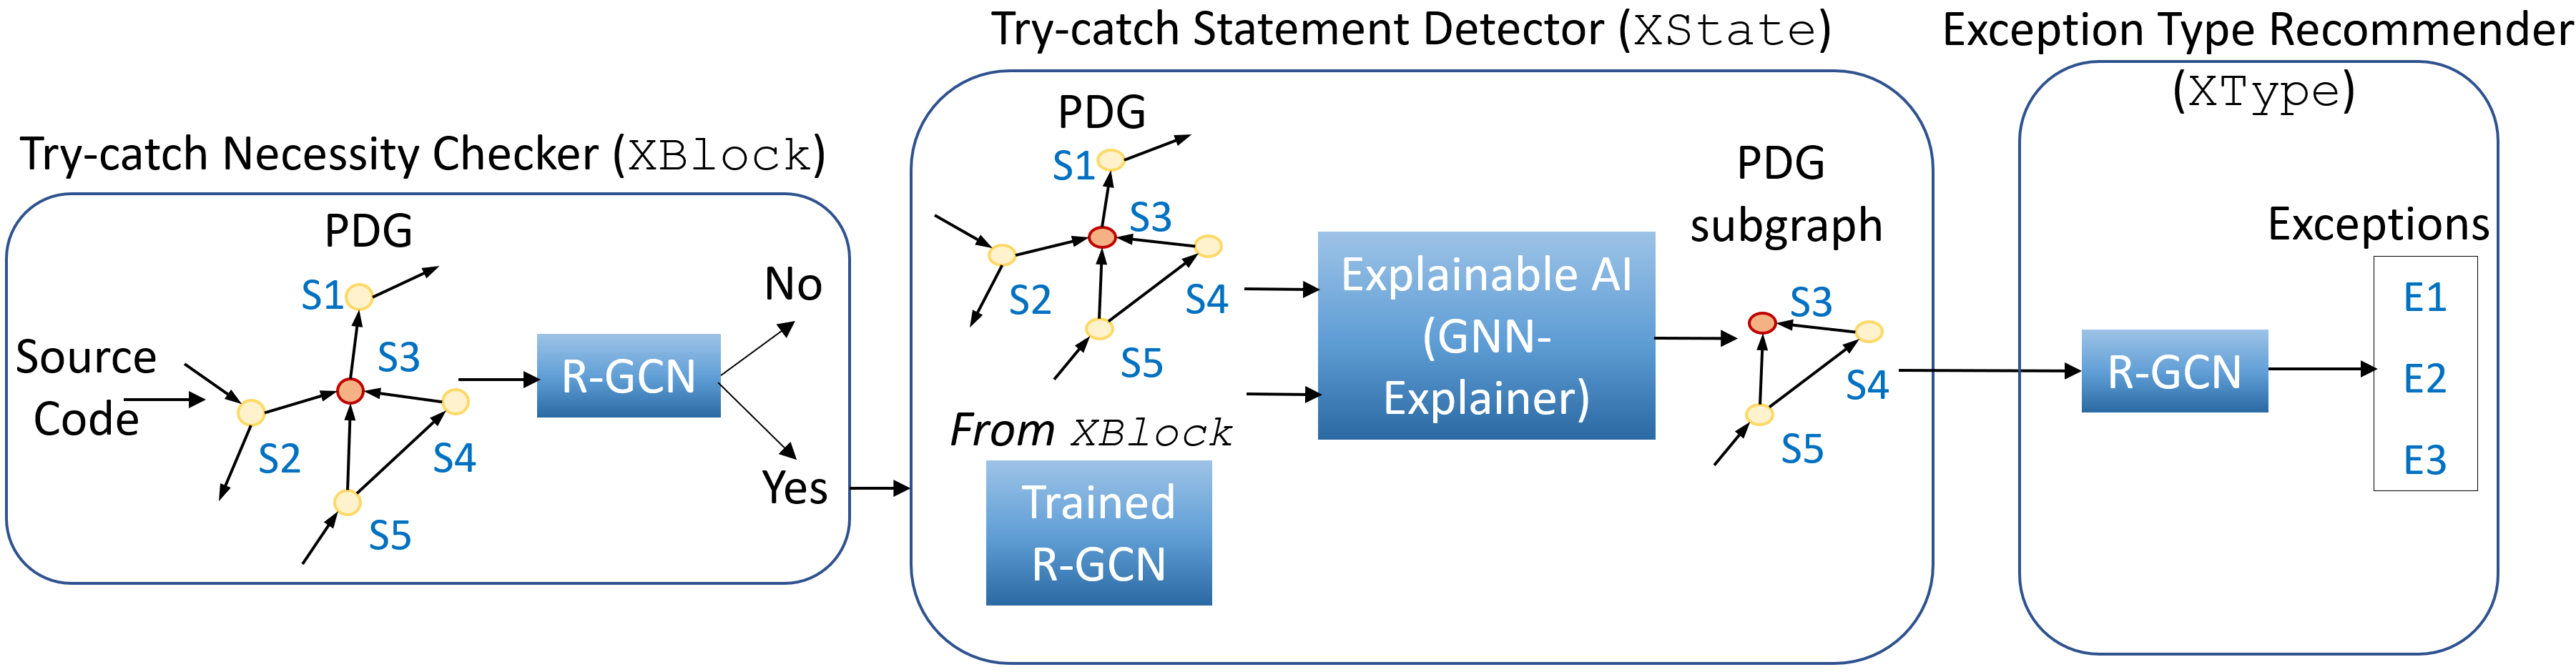
\includegraphics[width=5.4in]{overview-2.png}
\vspace{-10pt}
\caption{{\tool}: Architecture Overview}
\label{overview}
\end{center}
\end{figure*}

%Let us present the overview of our approach.

Given an input code snippet, we first split it by lines and concatenate them using a special token <SEP>. Then, we use the tokenizer from Pre-Trained CodeBERT to tokenize this concatenated string into sub-tokens and get the vector representation for each sub-token, as CodeBERT has been shown to have produced code representations that embed both the syntactic and semantic information. In the training phase, the input is all but the statements related to try-catch in a method body, while in the prediction phase, the input can be any code snippet that is part of a method body. 

The goal is to learn useful vector representations for a code snippet as a whole and for each statement in it so as to help the three downstream tasks. For each downstream task, we design a module , or block as we refer to it, in order to carrying out the specific learning task. The three blocks are XBlock, XState and XType. XBlock is for deciding whether the input code snippet needs any try-catch. If there are exceptions that need to be caught, XBlock outputs YES; otherwise, XBlock outputs NO. The second block is XState, where labelling technique is used to capture the statements in each try-block. In the training phase, we know whether the input contains try-block. If no try-block exists, we skip XState (and XType); In the prediction phase, we do not enter this block (and XType) if XBlock has output NO. The third block XType is for predicting which exceptions to catch for each try-block. The prediction is made on top of a vector representation of the try-block that is attained by composing individual vector representation of each statement in the try-block. In the training phase, we know which statements should be put in the same try-block as ground truth, while in prediction phase, we use the labelling results from XState to group statements into try-blocks. 

% In general, {\tool} has three main components. The first
% component, {\xblock}, aims to check if it is necessary to have a
% \code{try-catch} block for a given code snippet $C$. We extract the
% program dependence graph (PDG) from the source code using
% DeepPDA~\cite{icse23} that is capable of generating the PDG for any
% (in)complete code snippet. The PDG is used as an input for a
% Relational Graph Convolutional Network (R-GCN)~\cite{rgcn}, which acts
% as a classifier for {\xblock}. During training, we use the complete
% source code in the open-source projects in which each positive sample
% contains at least a \code{try-catch} block, and each negative sample
% does not contain any. If there are multiple consecutive blocks, we
% split them into individual ones. During prediction, {\xblock} uses the
% trained R-GCN model to predict whether the code snippet $C$ needs a
% \code{try-catch} block or not.

% In the case that the code snippet $C$ needs a \code{try-catch} block,
% the second component, {\xstate}, is aimed to detect which statements
% in $C$ that need to be placed into a \code{try-catch} block.  We model
% this task as an explanation task for {\xblock}. {\xstate} takes as
% input: 1) the PDG of the given code snippet, and 2) the trained R-GCN
% model for the \code{try-catch} necessity checker ({\xblock}), together
% with the classification result ``Yes'' from that R-GCN model of
% {\xblock}. {\xstate} leverages GNNExplainer~\cite{GNNExplainer}, a
% graph-based, Explainable AI model to decide the statements in the PDG
% that are most decisive and relevant to the reason why the code snippet
% $C$ is required to have a \code{try-catch} block. During training, in
% a positive sample, the statements in a \code{try-catch} block are
% marked as positive, and the ones outside of the block as negative. All
% the statements in a negative sample are marked as negative. During
% prediction, the output of GNNExplainer is a list of statements in
% $C$ (e.g., $S_3$, $S_4$, $S_5$) that made the R-GCN model in {\xblock}
% to decide the need of a \code{try-catch} block. We consider them as
% the statements to be in a \code{try-catch} block.

% The third component is the exception type recommender, {\xtype}.
% During training, the exception types in a \code{try-catch} block in
% the positive samples are used as the labels. During prediction,
% {\xtype} takes as input the result from GNNExplainer, which is the
% subgraph of the PDG of the given source code $C$. Another R-GCN model
% is used and acted as a classifier for all the exception
% types.


\section{{\xblock}: \code{Try-Catch} Necessity Checker}
\label{xblock:sec}

\begin{figure}[t]
 	\centering
 	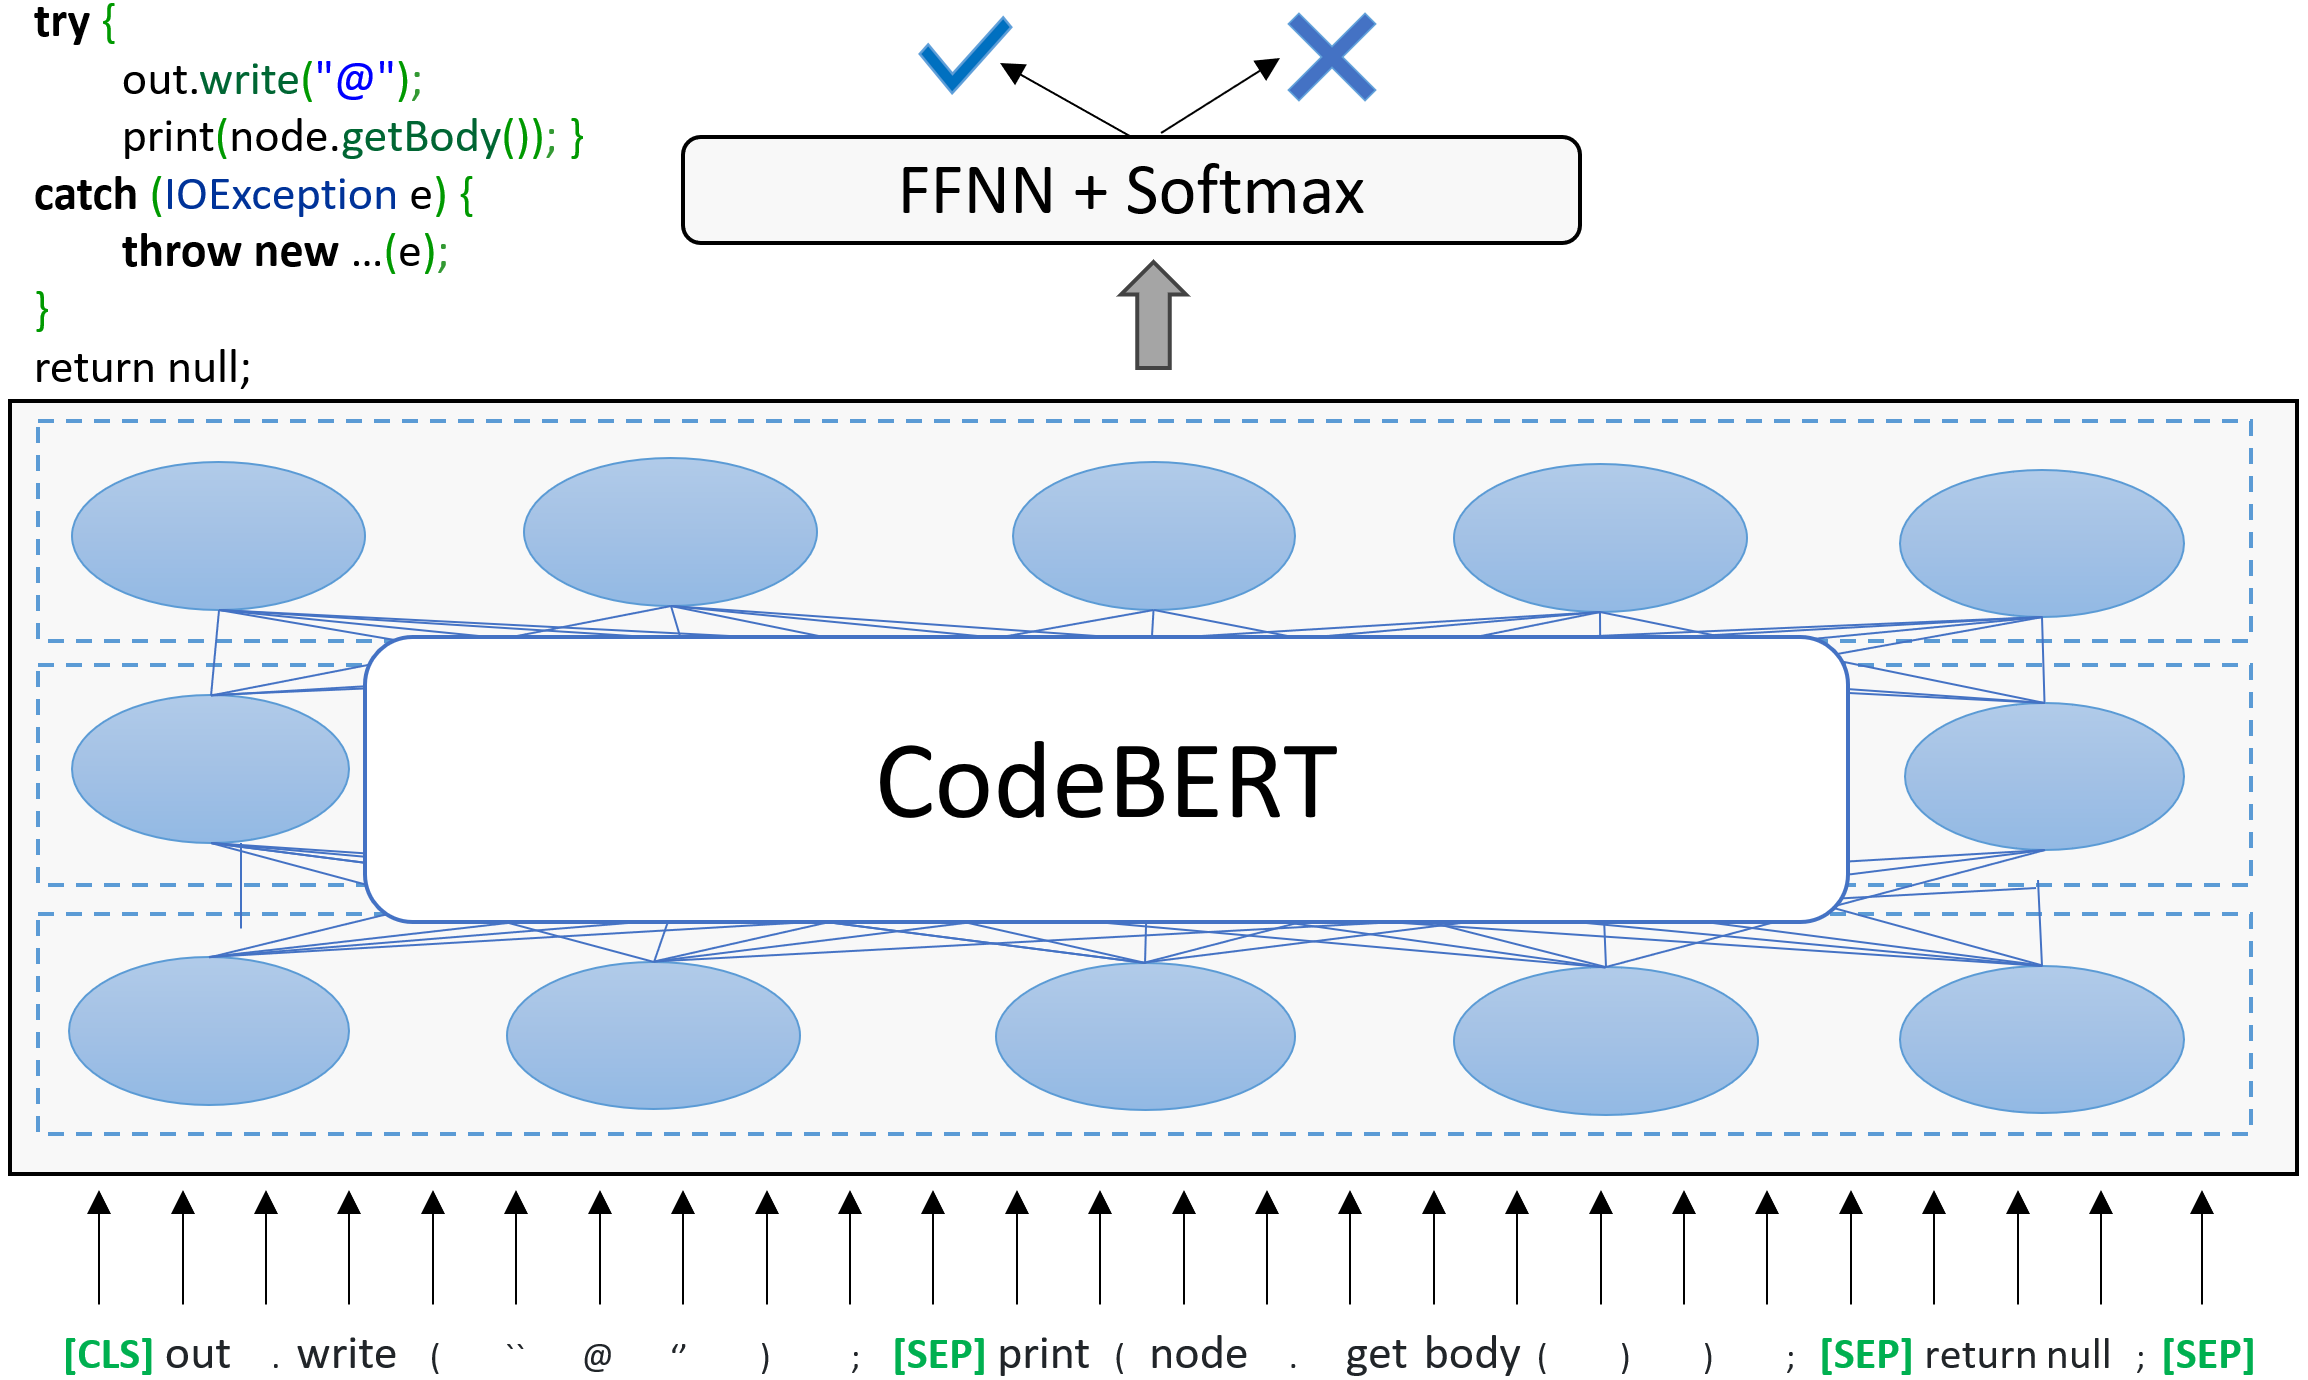
\includegraphics[width=3.4in]{xblock-6.png} %xblock-4
        \vspace{-20pt}
 	\caption{\code{Try-catch} Necessity Checker ({\xblock})}
 	\label{fig:xblock}	
\end{figure}

Figure~\ref{fig:xblock} illustrates {\xblock}'s architecture.  Given
an input code snippet, {\xblock} first splits it into the statements
(Figure~\ref{fig:xblock}). Each statement is then tokenized into
sub-tokens using CodeBERT's tokenizer. We use a special separator
token \texttt{[SEP]} to concatenate the tokenized statements, and add
a \texttt{[CLS]} token at the beginning of the code snippet. As in
CodeBERT, we take that \texttt{[CLS]} token to be the representation
of the entire code snippet.

We fine-tune a CodeBERT (MLM)~\cite{codebertMLM} for this task.
%Given the good performance of CodeBERT on many code-related downstream
%tasks,
We expect it to be able to learn the dependencies among statements
with API elements that would signal the need of exception
handling. Importantly, by providing the code snippet, we expect to
leverage the code context in which the API elements are used with
regard to one another. For example, in Figure~\ref{overview}, CodeBERT
is expected to learn that the APIs \code{newBufferedReader} of the
class \code{Files} and \code{readLine} of the class
\code{BufferedReader} are often used together in API usages and they
require \code{IOException}. For the input incomplete code,
CodeBERT is expected to learn such relations/connections to avoid name
ambiguity and to connect them with the exception types.

During training, as we use one CodeBERT, all three modules
(Sections~\ref{sec:xstate} and~\ref{sec:xtype}) contribute to the
signal for updating the model's parameters (multi-tasking). In
{\xblock}, we feed the vector representation of the \texttt{[CLS]}
token to a linear layer (Feed-forward neural network - FFNN) and use a
softmax function to learn the decision as to whether the input code
needs to be placed in a \code{try-catch} block.

%handle any exceptions.

% \begin{figure}[t]
% 	\centering
% 	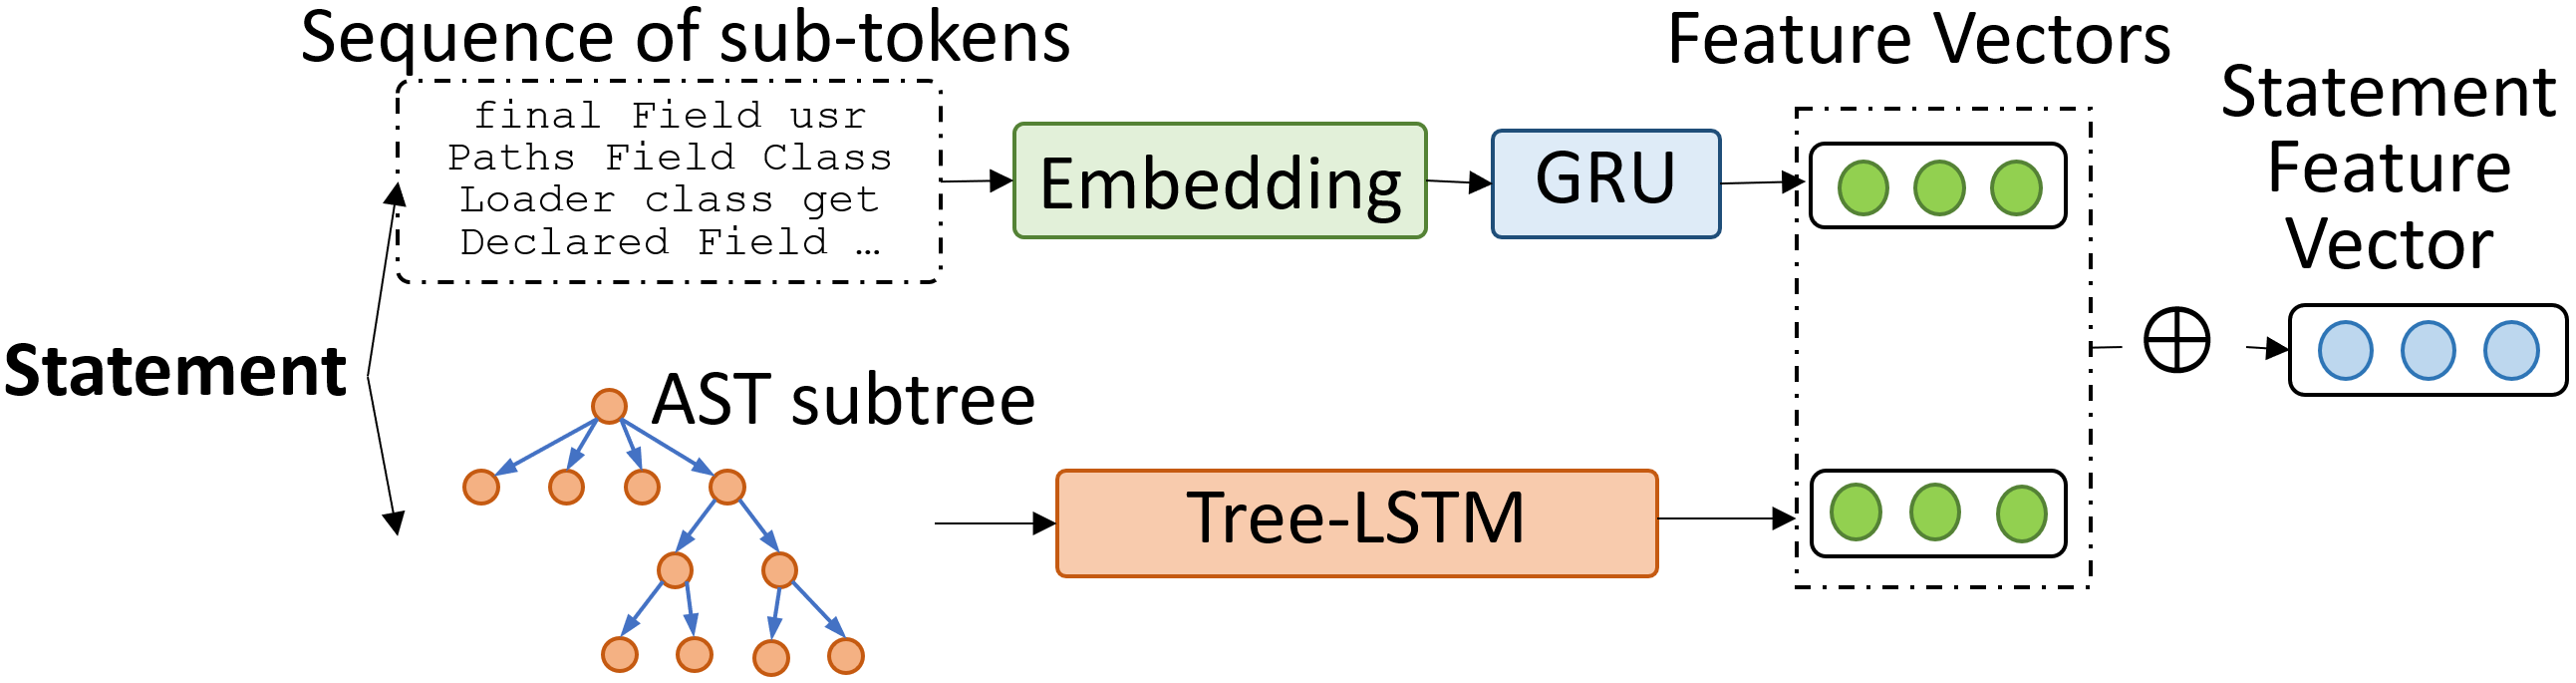
\includegraphics[width=3.2in]{features-2.png}
%         \vspace{-0.08in}
% 	\caption{Code Representation Learning for Statement}
% %        \vspace{-0.05in}
% 	\label{fig:feature}	
% \end{figure}

% %Tien
% %This section describes our graph-based {\xblock} model.

% We first explain how {\xblock} builds the context-aware representation
% learning for the given code, and uses such learned vectors to decide
% if the presence of \code{try-catch} block is needed using
% R-GCN~\cite{rgcn}.

% \subsection{Code Representation Learning}
% \label{replearn:sec}

% Let us explain how we build the vectors for code features
% (Figure~\ref{fig:feature}). We aim to capture the lexical and
% structural features for a statement, while PDG captures the program
% dependencies among statements.

% \vspace{-1pt}
% \subsubsection{Sequence of Sub-tokens of a Statement}

% At the lexical level, a statement is represented via a sequence of the
% sub-tokens. The sub-token granularity has been shown to have higher
% regularity than the tokens~\cite{icse20-methodname}. Each statement is
% tokenized using CamelCase or Hungarian convention. Then, only
% variables, methods, fields, and class' names are kept. The sub-tokens
% with one character are removed to avoid noises. In
% Figure~\ref{fig:example1} at line 2, we collect the sequence of
% sub-tokens as follows: \code{final}, \code{Field}, \code{usr},
% \code{Paths}, etc. We use a word embedding technique~\cite{glove2014}
% to build the vectors for the sub-tokens, together with Gate Recurrent
% Unit (GRU)~\cite{chung2014empirical} to build the feature vector for
% the sequence of sub-tokens for a statement (Figure~\ref{fig:feature}).


% \vspace{-1pt}
% \subsubsection{Code Structure of a Statement}

% At the syntactic level, we aim to capture the code structure via the
% AST. {\tool} parses the code and extracts the AST subtree for the
% given statement, and then feeds it to the Tree-LSTM
% model~\cite{tai2015improved}, which produces a feature vector to
% capture the structure of the statement (Figure~\ref{fig:feature}). If
% the given code is incomplete, we use PPA~\cite{dagenais-oopsla08}, a
% partial program analysis tool to produce the AST for the code in a
% best-effort fashion.


% \subsection{\code{Try-catch} Necessity Checker with R-GCN}
% \label{model:sec}



% Figure~\ref{fig:gcn} illustrates how we use the R-GCN model~\cite{rgcn} to
% detect if a \code{try-catch} block is needed.
% %The rationale is that FA-GCN can deal well with the graphs with sparse
% %features (not all the statements share the same properties), and
% %potentially noisy features in a PDG.
% First, the code is processed by DeepPDA~\cite{icse23}, which is
% capable of parsing any (in)complete code to build the PDG. The
% R-GCN, similar to CNN in image processing, performs a sliding
% window along the nodes in the graph. A window for a node consists of
% its neighboring nodes in the PDG.
% %Similar to CNN using the filter on an image, FA-GCN performs sliding
% %a small window along all the nodes (statements) of the PDG. For
% %example, in Figure~\ref{fig:gcn}, the window marked with A for the
% %node $S27$ consists of itself and the neighboring statements/nodes
% %$S6$, $S22$, $S25$, and $S29$. Another window (marked with B) is for
% %the node $S23$, including itself and the neighboring nodes: $S22$ and
% %$S25$.
% To process a window, the model generates the feature representation
% matrix for the node at the center using the procedure described in
% Figure~\ref{fig:feature}.
% %For example, for the window centered at $S27$, it generates the
% %feature vector $F_{S27}$ for $S27$, using the process explained in
% %Figure~\ref{fig:feature}.
% From the representation vectors for all statements (nodes), the R-GCN
% model will produce the outputs at the output layer. The R-GCN model
% connects all of its outputs to a fully connected layer to transform
% the matrix into a vector $V_C$ to represent the given code
% $C$. {\tool} then performs classification by using a softmax function
% on $V_C$ to decide if a \code{try-catch} block is needed for the
% source code $C$.





\section{Try-Catch Statement Detector via Explainable AI}
\label{interpretation:sec}

This section explains {\xstate} and how we leverage an Explainable AI
model in GNNExplainer~\cite{GNNExplainer} to detect what statements in
the given code snippet need to be placed in a \code{try-catch} block
provided that {\xblock} had decided the necessity of such a block.

%Tien
{\xstate} takes the following as inputs: 1) the PDG ($G_C$) of the
given code $C$, 2) the trained R-GCN model for {\xblock}, along with
the positive detection result $\mathcal{V}$ with the prediction score.
Figure~\ref{fig:GNNEX} displays an illustration of the process in
{\xstate}.

% Let us explain how we use GNNExplainer~\cite{GNNExplainer} to build
%our graph-based interpretation. The input includes the trained FA-GCN
%model, the PDG ($G_M$) of the method $M$, and the detection result
%$\mathcal{V}$ or $\mathcal{NV}$, and prediction score.

%Figure~\ref{fig:GNNEX} illustrates our process for the case of
%$\mathcal{V}$ (Vulnerable) (the case of $\mathcal{NV}$ is done
%similarly).



%The interpretations include 1) a crucial sub-graph $\mathcal{G}_M$,
%corresponding to the PDG sub-graph consisting of statements relevant
%to the vulnerability, and 2) a subset of crucial features
%$\mathcal{X}_M$, corresponding to the set of variables involving to
%the vulnerability.

To decide the statements in the given code to be placed in a
\code{try-catch} block, we aim to determine the statements that are
most decisive and crucial for the {\xblock} model in deciding its
outcome of ``Yes'' (i.e, {\xblock} decides that the snippet must be
placed in a \code{try-catch} block). Therefore, we formulate that as
the following problem: finding a sub-graph $\mathcal{G}_C$ in the PDG
$G_C$ for $C$ that minimizes the difference in the prediction scores
between using the entire graph $G_C$ and using the minimal graph
$\mathcal{G}_C$. To do so, we leverage the Explainable AI model,
GNNExplainer~\cite{GNNExplainer}. It uses a masking technique in which
instead of searching for that minimal subgraph, it learns the {\em
  edge-mask} set $EM$ of the edges and the {\em feature-mask} set $FM$
of the features. Learning those two sets $EM$ and $FM$ helps derive
the explanation sub-graph $\mathcal{G}_C$ and the set of crucial
feature $\mathcal{X}_C$ by masking-out the edges in $EM$ and the
feature in~$FM$ from $G_C$ and $X_C$:
\begin{equation}\label{eq:11}
\mathcal{G}_C = G_C \bigodot EM
\end{equation}
\begin{equation}\label{eq:12}
\mathcal{X}_M = X_M \bigodot FM
\end{equation}
$\bigodot$ is used to denote ``masking-out''.

%To derive the interpretations, the key goal is to find a sub-graph
%$\mathcal{G}_M$ in the PDG $G_M$ of the method $M$ that minimizes the
%difference in the prediction scores between using the entire graph
%$G_M$ and using the minimal graph $\mathcal{G}_M$. To do so, we use
%GNNExplainer with the {\em masking technique}~\cite{GNNExplainer},
%which treats the searching for the minimal graph $\mathcal{G}_M$ as a
%learning problem of the {\em edge-mask} set $EM$ of the edges.  The
%idea is that learning $EM$ helps {\tool} derive the interpretation
%sub-graph $\mathcal{G}_M$ by masking-out the edges in $EM$ from $G_M$
%(``masked-out'' is denoted by
%$\bigodot$): \begin{equation}\label{eq:11} \mathcal{G}_M = G_M
%\bigodot EM \end{equation}

Figure~\ref{fig:GNNEX} illustrates the principle. Note that the
trained R-GCN model in {\xblock} had decided that a \code{try-catch}
block is needed for the given code (in which the entire original PDG
was used as input). When an edge-mask set is applied, some of the
edges (and the inducing nodes) are masked. With the new graph being
used as~the new input, if the trained R-GCN model in {\xblock}
produces ``Yes'' as the result, i.e., {\em the classification does not
change, then the edges in the edge-mask set are not important}. Thus,
they will not be included in the explanation graph $\mathcal{G}_C$. If
the trained R-GCN model in {\xblock} with the new input graph produces
``No'' as the result, i.e., {\em the classification does change from
``Yes'' to ``No'', then those edges in the edge-mask set are important
to the model, thus, being included in the explanation graph
$\mathcal{G}_C$}. Similar logic is applied to include or exclude the
features in the {\em feature-mask} $FM$.



%Tien Figure~\ref{fig:GNNEX} illustrates GNNExplainer's principle. As
%an edge-mask set is applied, GNNEXplainer checks if the FA-GCN model
%produces the same result~(in this case the result is
%$\mathcal{V}$). If yes, the edge in the edge-mask is not important
%and is not included in $\mathcal{G}_M$. Otherwise, the edge is
%important and included in $\mathcal{G}_M$.  Because the numbers of
%possible sub-graphs and the edge-mask sets are untractable,
%GNNExplainer uses a learning approach for the edge-mask $EM$.

%\begin{equation}\label{eq:12}
%\mathcal{X}_M = X_M \bigodot FM
%\end{equation}

%For example, as you can see in figure \ref{fig:GNNEX}, when the
%GNNExplainer get the whole PGD $G_m$, it starts to use the
%\textit{edge-mask} $EM$ and \textit{feature-mask} $FM$ to mask some
%edges and features.  As you can see in the second row of the figure,
%after masked some edges from $G_m$ to generate a graph $G'_m$,
%GNNExplainer use the detection model to check the new graph to see
%how the detection result changes. If the result has been influenced a
%lot, it means that the masked edges are important for the detection
%result. If not, it means that the masked edges are not important for
%the detection result. It is similar for the \textit{feature-mask}
%$FM$.  Because in the last step, we could get $F_{v}$ for each
%statement $v$ and $F_{v}$ have the same dimension, $FM$ masks the
%features in the same position in $F_{v}$ for each statement $v$ and
%then use detection model to evaluate the importance of the masked
%features just as the edges. As you can see in figure \ref{fig:GNNEX},
%$FM$ masked the second and the 4th feature for each statement in this
%example.

\begin{figure}[t]
	\centering
	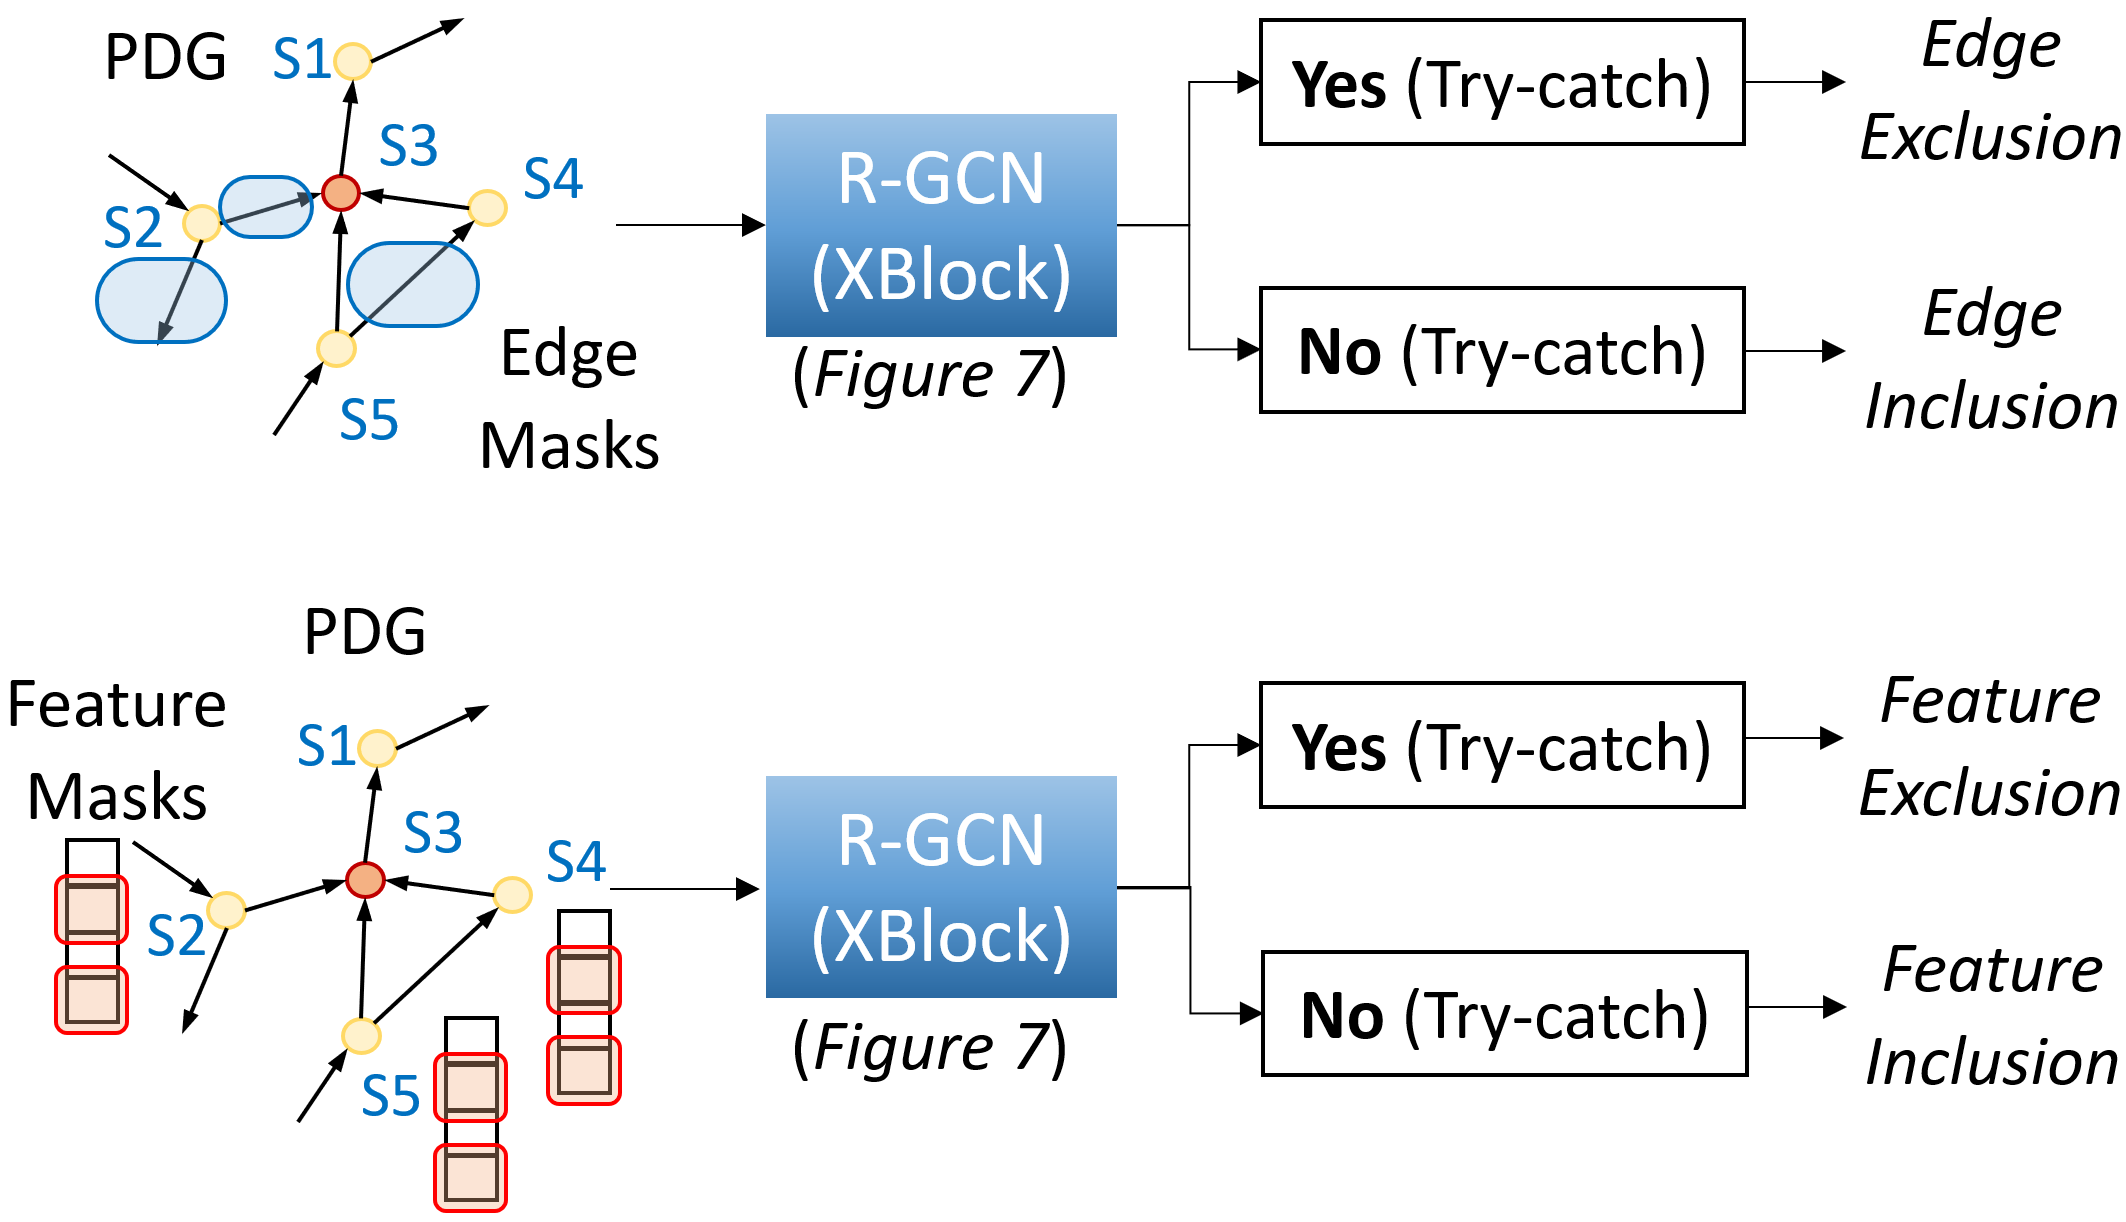
\includegraphics[width=3.2in]{XAI.png}
        \vspace{-0.06in}
	\caption{Masking to Derive Explanation Sub-Graphs with Statements in a Try-Catch Block}
        \vspace{-0.06in}
	\label{fig:GNNEX}	
\end{figure}

%\begin{align}\label{maineq}
%\nonumber
%\max_{\mathcal{G}_M} MI(Y,(\mathcal{G}_M,\mathcal{X}_M)) = H(Y) - H(Y|G=\mathcal{G}_M,X=\mathcal{X}_M)
%\end{align}

%to minimizing conditional entropy
%$H(Y|G=\mathcal{G}_M,X=\mathcal{X}_M)$

%\begin{equation}
%  \label{eq2}
%-\EX_{Y|\mathcal{G}_M,
%  \mathcal{X}_M} [log P_{FA-GCN} (Y|G=\mathcal{G}_M,X=\mathcal{X}_M)]
%  \end{equation}

%\begin{equation}
%  \label{eq3}
%  \min_{\mathcal{G}} \EX_{\mathcal{G}_M \sim \mathcal{G}} H(Y|G=\mathcal{G}_M,X=\mathcal{X}_M)
%\end{equation}
%\begin{equation}
%  \label{eq4}
%  \min_{\mathcal{G}} H(Y| G=\EX_{\mathcal{G}}[\mathcal{G}_M], X=\mathcal{X}_M)
%\end{equation}
%\nonumber

Because the numbers of possible sub-graphs, edge-mask sets, and
feature-mask sets are untractable, GNNExplainer uses a learning
approach for $EM$ and $FM$. It aims to maximize the mutual information
(MI) between the minimal graph $\mathcal{G}_C$ and the input
PDG~$G_C$~\cite{GNNExplainer}:
\begin{equation}\label{maineq}
\max_{\mathcal{G}_C} MI(Y,\mathcal{G}_C) = H(Y) - H(Y|G=\mathcal{G}_C)
\end{equation}
$Y$ is the outcome decision by the trained R-GCN model. Thus, the
entropy term $H(Y)$ is constant for the trained R-GCN
model.

Maximizing the $MI$ value for all $\mathcal{G}_C$s is equivalent
to minimizing conditional entropy $H(Y|G=\mathcal{G}_C)$, which by
definition of conditional entropy can be expressed~as
\begin{equation}
  \label{eq2}
-\EX_{Y|\mathcal{G}_C}
  [log P_{R-GCN} (Y|G=\mathcal{G}_C]
\end{equation}
This conditional entropy is a measure of how
much uncertainty remains about the outcome $Y$ when we know
$G=\mathcal{G}_C$.
%
%GNNEXplainer also limits the size of $\mathcal{G}_C$ by $K_C$, {\em
%  i.e.}, taking $K_C$ edges that give the highest mutual information
%with the prediction outcome $Y$.
%
%Direct optimization of the formula(~\ref{eq2}) is not tractable, thus,
%GNNExplainer treats $\mathcal{G}_C$ as a random graph variable
%$\mathcal{G}$. The objective in Equation(~\ref{eq2}) becomes:
%\begin{equation}
%  \label{eq3}
%  \min_{\mathcal{G}} \EX_{\mathcal{G}_C \sim \mathcal{G}} H(Y|G=\mathcal{G}_C)
%\end{equation}
%\begin{equation}
%  \label{eq4}
%  \min_{\mathcal{G}} H(Y| G=\EX_{\mathcal{G}}[\mathcal{G}_C])
%\end{equation}
%From Equation~\ref{eq3}, we obtain Equation~\ref{eq4} with Jensen's
%inequality.  The conditional entropy in Equation~\ref{eq4} can be
%optimized by replacing $\EX_{\mathcal{G}}[\mathcal{G}_C]$ to be
%optimized by masking with $EM$ on the input graph $G_C$.  Now, we can
%reduce the problem to learning the mask $EM$.  Similar logic is
%applied to $FM$.

More details can be found in~\cite{GNNExplainer}. The resulting
sub-graph $\mathcal{G}_C$ is used to derive the statements to be
placed in a \code{try-catch} block. Note that, we can set the
statements to be consecutive.


\section{Exception Type Recommender}
\label{sec:type}

\begin{figure}[t]
\begin{center}
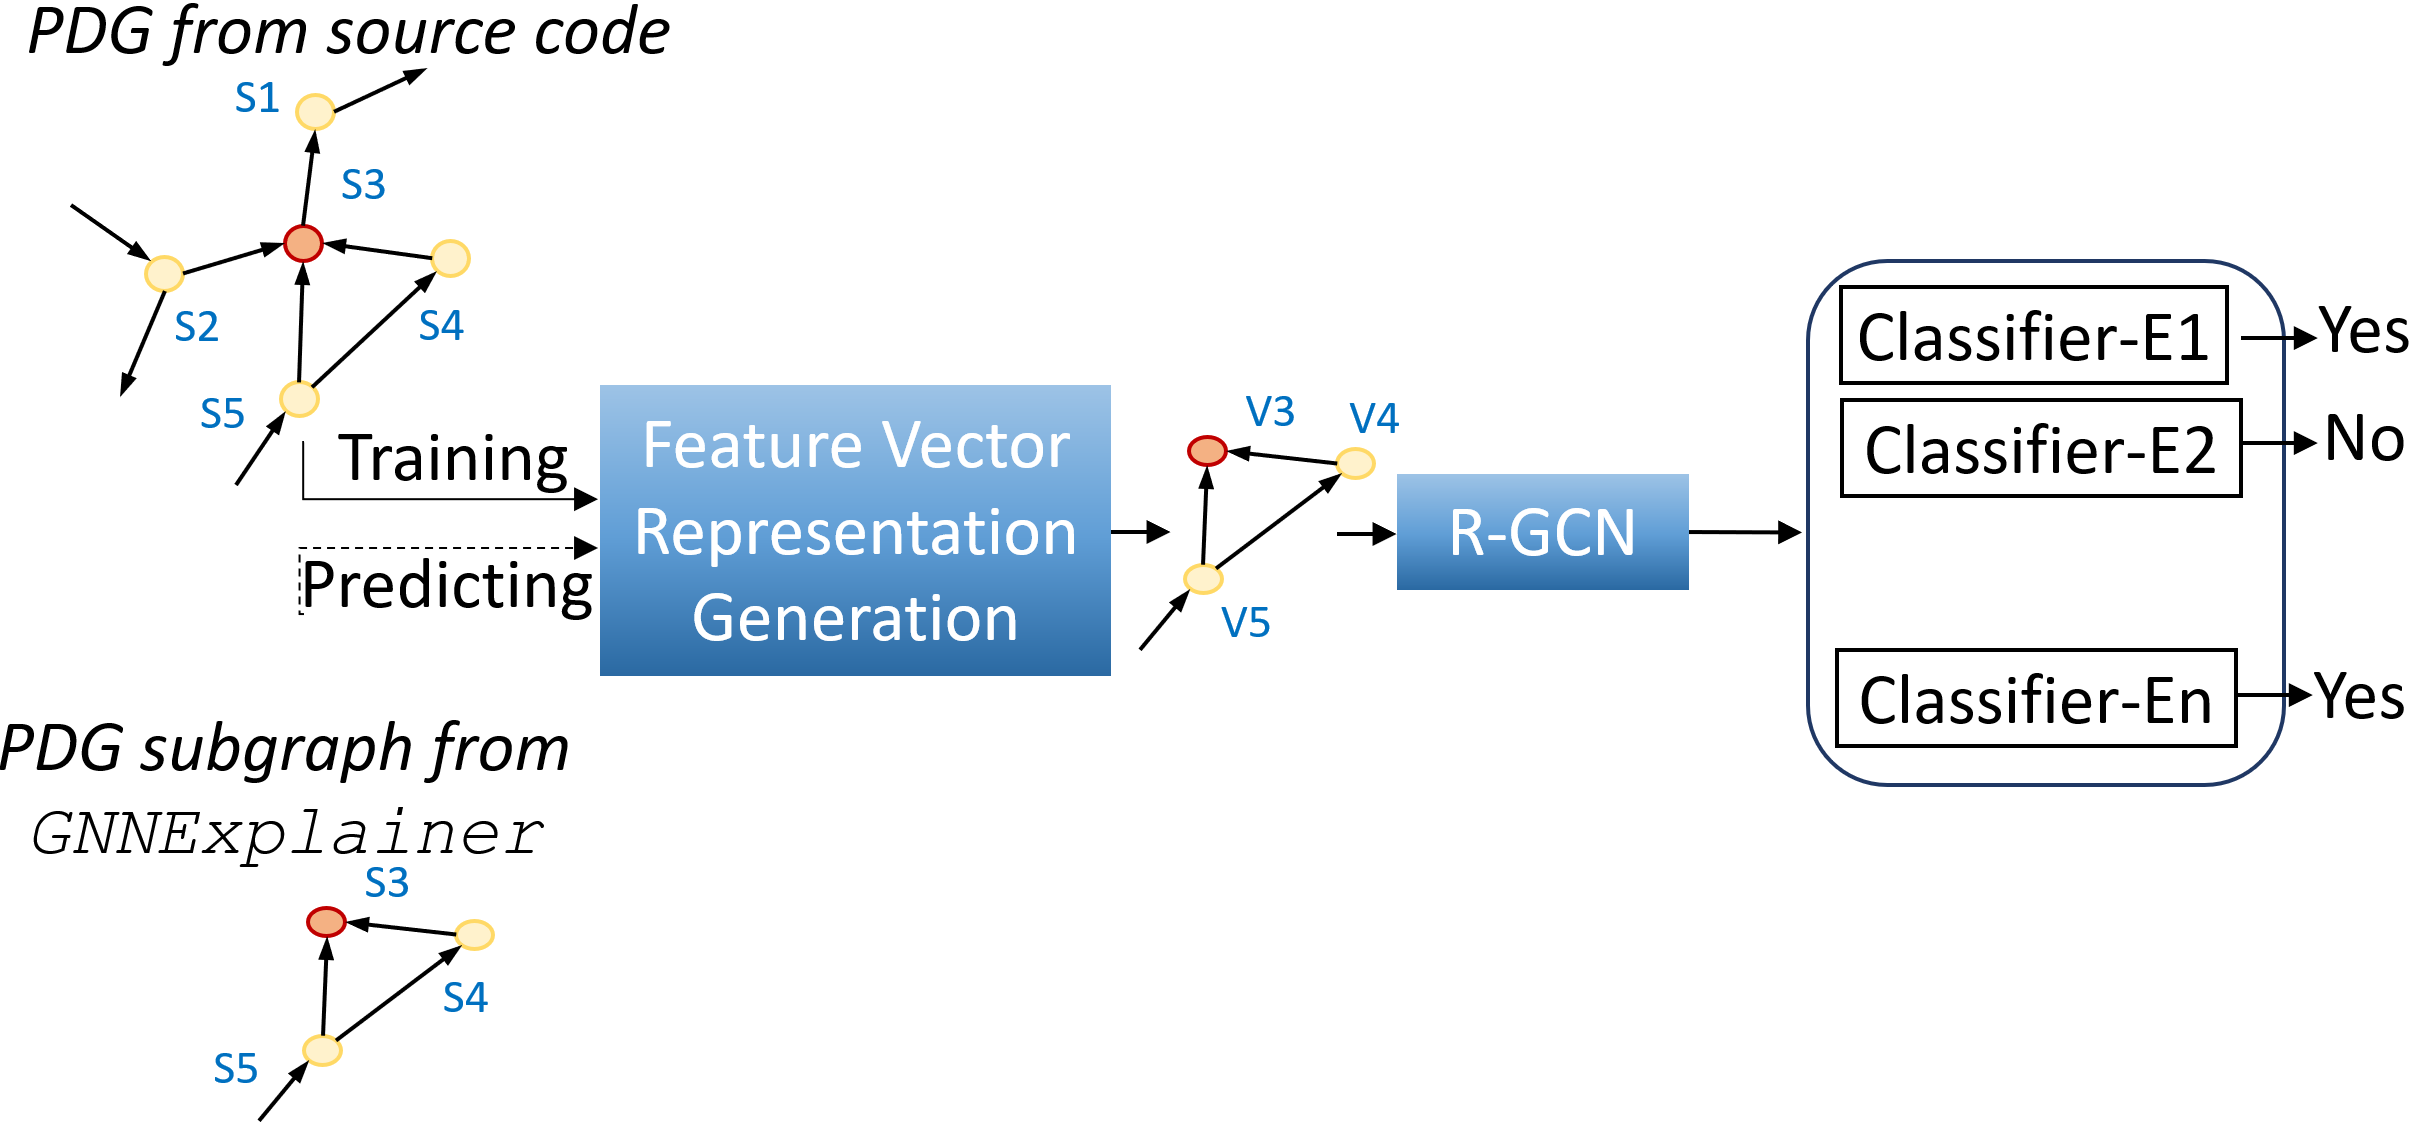
\includegraphics[width=3in]{xtype}
\vspace{-10pt}
\caption{Exception Type Recommendation ({\xtype})}
\label{fig:xtype}
\end{center}
\end{figure}

This section describes {\xtype} that recommends the exception types to
be handled in the \code{catch} clause for the given code, after it was
determined to require a \code{try-catch} block and some of its
statements was determined to be placed in that block.

We use another R-GCN model that acts as a classifier for different
exception types (Figure~\ref{overview}). For training, the source code
with \code{try-catch} blocks is used as input. {\tool} parses and
processes them in the same way to build the feature vector
representations for the statements as in {\xblock}
(Figure~\ref{fig:feature}). However, in prediction, the input is the
sub-graph $\mathcal{G}_C$ of the PDG because the GNNExplainer already
determined that those statements in that sub-graph need to be placed
in a \code{try-catch} block. In this case, the feature vectors are
also built in the same way as in Figure~\ref{fig:feature}. The R-GCN
model processes the input (sub)graph in a similar manner as in
Figure~\ref{fig:gcn} except the post-process on the output of that
model.  Instead of connecting the output vector of the R-GCN model to
a fully connected layer, we feed that output to multiple softmax
functions to act as the classifiers for multiple exception types in
the dictionary. Each classifier is responsible for one exception type.
We could limit the maximum number of exception types. The positive
output from a classifier indicates the presence of the corresponding
exception type in the \code{catch} clause.


%\section{Empirical Evaluation}
\label{sec:eval}

\subsection{Research Questions}

We conducted several experiments to evaluate {\tool}. We seek to
answer the following questions:

\vspace{2pt}
%\noindent \textbf{RQ\textsubscript{1}. [Effectiveness on Java code]
%  (Intrinsic Evaluation).} {\em How accurate is {\tool} in generating
%  CFG/PDGs for Java code in general and in different dependency
%  types?}

\noindent \textbf{RQ\textsubscript{1}. [Effectiveness on Try-Catch
    Necessity Checking]} {\em How accurate is {\tool} in predicting
  whether a given code snippet needs to have a \code{try-catch}
  block?}
    
%            program-dependency edges generated by \tool for Java code?
%            How accurately does \tool predict different types of
%            control-flow and program-dependency edges for Java code?}


\vspace{2pt}
\noindent \textbf{RQ\textsubscript{2}. [Effectiveness on Try-Catch
    Statement Detection].} {\em How accurate is {\tool} in predicting
  which statements in a given code snippet needs to be placed in a
  \code{try-catch} block?}

%\vspace{2pt}
%\noindent \textbf{RQ\textsubscript{4}. [Ablation Study on C/C++
%    code].}  {\em How do the different components in \tool contribute to
%  model performance?}

\vspace{2pt}
\noindent \textbf{RQ\textsubscript{3}. [Effectiveness on Exception Type Recommendation].}
{\em How accurate is {\tool} in recommending what exception types need to be handled in the \code{catch} clause of a \code{try-catch} block?}

\vspace{2pt}
\noindent \textbf{RQ\textsubscript{4}. [Dependency Probing].}
{\em How well {\tool} learn the dependencies among statements for grouping them into a \code{try-catch} block?}

\vspace{2pt}
\noindent \textbf{RQ\textsubscript{5}. [Usefulness on
    Exception-related Bug Detection].}  {\em How well does {\tool}
  detect exception-related bugs?}

\vspace{2pt}
\noindent \textbf{RQ\textsubscript{6}. [Ablation Study].} {\em How does
 fine-tuning improve {\tool}?}



\subsection{Empirical Methodology}

\subsubsection{Datasets}

%jodatime, jdk, Android, xstream, gwt, hibernate

We conducted experiments on two datasets: 1) {\em Github dataset}
for intrinsic evaluation on exception handling recommendation tasks
({\xblock}, {\xstate}, {\xtype}), and 2) {\em FuzzyCatch}
dataset~\cite{xrank-fse20} for extrinsic evaluation on
exception-related bug detection.
%
%FuzzyCatch dataset was provided by the authors of
%XRank/XHand~\cite{xrank-fse20}. We used FuzzyCatch dataset for our
%extrinsic evaluation.
%
We collected the Github dataset as follows. We first chose in Github
5,726 Java projects with the highest ratings that use
the following libraries: jodatime, JDK, Android, xtream, GWT, and
Hibernate. These are the well-established libraries that have been used
in several prior research on the topics related to
APIs~\cite{icse18,liveapi14}. We then selected the methods with at
least one \code{try-catch} block. 
%If there is one \code{try-catch}
%block, we take the body of the method as the code
%snippet. If there are multiple \code{try-catch} blocks in a method, we
%split the method into multiple code snippets by checking the above and
%below statements, one by one, starting from the closest one for each
%\code{try-catch} block, to verify if the statement is included in the
%other block. If not, we put it in the current code snippet. If yes, we
%finish the current one. 
In total, we have
153823 code snippets containing
\code{try-catch} blocks as positive samples. We also randomly selected
from the same Github projects the same amount of code snippets that do
not have any \code{try-catch} block as the negative samples.

For extrinsic evaluation, we used FuzzyCatch dataset, provided by the
authors of XRank/XHand~\cite{xrank-fse20}, which contains 750 samples
of methods with exception-related bugs (missing \code{try-catch}
blocks or missing catching some exceptions).  

%We also randomly selected from the projects in FuzzyCatch dataset the same amount of code snippets with no exception-related bugs as the negative samples.

%We have conducted our experiments to evaluate {\tool} on the dataset DeepEx that we collected, and the existing dataset FuzzyCatch provided in a prior work~\cite{nguyen2020code}.

%To build the dataset DeepEx, we first collect XXX methods from XXX Java projects. And then, we picked XXX methods that contain at least one try-catch block from all methods. To avoid the influence of multiple try-catch blocks, we split the methods into code snippets by checking the above and below statements, one by one, starting from the closest one for each try-catch block, to verify if the statement is included in the other try-catch block. If not, we put it in the current code snippet. If yes, we stop here and finish the code snippet.

%Following the steps mentioned above, we have XXX code snippets containing one try-catch block as positive data. Then, we randomly create the same amount of code snippets that do not contain a try-catch block as negative data from the Java projects we collected. So, in total, the DeepEx dataset includes XXX code snippets. As for the FuzzyCatch dataset, it includes 1,000 data, and all of them are positive data.


\subsubsection{RQ1. Effectiveness on Try-Catch Necessity Checking\\}

\indent {\em Baselines.} We compared {\xblock} against
XRank~\cite{xrank-fse20} (XRank is part of FuzzyCatch tool). XRank
computed the exception risk score for each API call.
%(i.e., the potential need of \code{try-catch} block).
If one score of a call in the snippet is higher than a threshold,
it is considered as needing a \code{try-catch} block.

{\em Procedure.} We used the Github dataset and randomly split both
the positive and negative sets into 80\%, 10\%, and 10\% of the code
snippets for training, tuning, and testing.

%We took all the code snippets from DeepEX and FuzzyCatch datasets. On
%the DeepEx dataset, we randomly split both the positive and negative
%data points into 80\%, 10\%, 10\%, in which 80\% of the code snippets
%as the training dataset, 10\% of the code snippets as the tuning
%dataset, and 10\% of the code snippets as the testing dataset for the
%baseline and {\tool}.

%THIS PART FOR RQ5
%----------------
%And on the FuzzyCatch dataset, we directly use
%the trained model from the DeepEx dataset and test it on the
%FuzzyCatch dataset for both the baseline and {\tool}.

{\em Tuning.} We tuned {\tool} with autoML~\cite{NNI} for the
following key hyper-parameters to have the best performance: (1) Epoch
size (50, 100, 150); (2) Batch size (32, 64, 128); (3) Learning rate
(0.001, 0.003, 0.005); (4) Vector length of feature embeddings and its
output (64, 128, 256); (5) Number of R-GCN layers (4, 6, 8).

{\em Metrics.} We use \textbf{Recall, Precision}, and {\bf F-score} to
evaluate the performance of the approaches. They are calculated as
$Recall = \frac{TP}{TP+FN}$, $Precision = \frac{TP}{TP+FP}$, $F$-score
$=$ $\frac{2*Recall*Precision}{Recall+Precision}$. $TP$: true
positive, $FN$: false negative, and $FP$: false positive.

\subsubsection{RQ2. Effectiveness on Try-Catch Statement Detection\\}

\indent {\em Baselines.} None. FuzzyCatch (XRank/XHand) does not have
this.

{\em Procedure.} We processed the Github dataset for this experiment
as follows. For the snippets that need \code{try-catch}, but were
predicted as not, we consider them as incorrect because the resulting
statements predicted from {\xstate} do not make sense for incorrect
{\xblock}'s detection. The snippets that do not need \code{try-catch},
but were predicted as yes, we also consider them as incorrect for the
same reason. Thus, for the evaluation of {\xstate}, we used the set of
code snippets that {\xblock} predicted correctly as needing a
\code{try-catch} block. We used the same data splitting scheme with
80\%, 10\%, and 10\% for training, tuning, and testing as in RQ1. Each code
snippet in the testing set and the trained R-GCN model in {\xblock}
are the input of the GNNExplainer model in {\xstate} in this
experiment.

%In this RQ, \tool is evaluated on the DeepEx dataset. Because only the data points that are predicted as needing a try-catch block, the \tool will run the try-catch statement detection on them. To fully use the dataset and evaluate \tool on more data, here we estimate the accuracy of RQ1 prediction is 100\% which means that we use all positive data in DeepEx dataset as the data we use in this RQ. We do the same data split as RQ1 to train, validate and test the model performance.

{\em Tuning.} We used the same parameters as in
GNNExplainer~\cite{GNNExplainer}. It also has a parameter on the limit
of the number $N$ of the nodes in the explanation sub-graph. We
varied $N$ from 1 to 10. The average number of statements in a
\code{try-catch} block in Github dataset is 5.9.

%We tuned {\tool} in this RQ by testing different node number limits for generated sub-graph. The range of the node number limit we tested is from $1$ to $10$ nodes.

{\em Metrics.} If {\xstate} predicts for a statement correctly if it
is in a \code{try-catch} block or not, we count it as a correct case.
Otherwise, it is an incorrect one. \textbf{Accuracy} is
defined as the ratio between the number of correct statements over the
total number of statements.

%For each statement in the try-catch block, if
%\tool included it in the generated sub-graph, we think the prediction
%on it is correct. Otherwise, it is incorrect. The Accuracy is
%calculated as $Accuracy = \frac{Correct}{Correct + Incorrect}$.

\subsubsection{RQ3. Effectiveness on Exception Type Recommendation\\}

{\em Baselines.} None. XRank/Xhand do not support this feature.

%We compared {\tool} against the state-of-the-art exception type recommendation approach XRank~\cite{nguyen2020code}.

{\em Procedure.} We processed the Github dataset for this experiment
in the same manner as in RQ2 because the result of {\xtype} (i.e.,
what exception types need to be in the \code{catch} clause) makes
sense only when one knows that the given code snippet needs to have a
\code{try-catch} block. Thus, for the evaluation of {\xtype}, we used
the set of code snippets that {\xblock} predicted correctly as needing
a try-catch block. We used the same splitting as RQ2. The exception
types in the \code{catch} clauses are used as the labels.

%In this RQ, \tool is evaluated on the DeepEx dataset. Because only the data points that \tool can successfully predict all statements in the try-catch block successfully, the \tool will run the exception type prediction on them. Similarly, as RQ2, to fully use the dataset and evaluate \tool on more data, here we estimate the Accuracy of RQ2 prediction is 100\% which means that we use all positive data in DeepEx dataset as the data we use in this RQ. We do the same data split as RQ1 and RQ2 to train, validate and test the model performance.

{\em Tuning.} We tuned {\tool} with autoML~\cite{NNI} for the
key hyper-parameters to have the best performance as in RQ1 including
epoch size, batch size, learning rate, vector length, and R-GCN layers.
%(1) Epoch size (50, 100, 150); (2) Batch size (32, 64, 128); (3)
%Learning rate (0.001, 0.003, 0.005); (4) Vector length of feature
%embeddings and its output (64, 128, 256); (5) Number of R-GCN layers
%(4, 6, 8).

{\em Metrics.} Let us use $E$ and $P$ to denote the set of the
exception types in the oracle and the set of predicted
ones for one code snippet in the testing set. We aim to measure 1) how
precise {\tool} predicts the exception types ({\bf Precision}), i.e.,
how accurate the predicted types in $P$, and 2) how much {\tool} can
cover in its prediction with respect to the oracle ({\bf Recall}),
i.e., how much of $E$ that the predicted set $P$ can cover. Toward
measuring Precision and Recall, we define {\bf Hit-$n$} as the number
of the cases in which the predicted set $P$ contains
{\em at least} $n$ correct exception types, i.e., $P$ and $E$ overlaps
{\em at least} $n$ exception types regardless of the sizes of both
sets.

In Github dataset, more than 98.1\% of the code snippets have 1--3
exception types in a \code{catch} clause. Thus, we compute Hit-$n$,
Precision, and Recall for the size of $E$ (|$E$|) from 1--3 and 3+,
and for the size of $P$ (|$P$|) from 1--3 and 3+.
%
When computing Recall, we use the set $E$ as the basis. Recall at a
size $N_E$ of $E$ is computed as the ratio between Hit-$n$ at that
size and the total number of cases with that size $N_E$. We compute
Recall for all $N_E$ = 1--3, and 3+, and $n$=1--$N_E$. We also define
{\bf \code{Hit-All}$_{Rec}$} as \code{Hit}-$n$ when the number $n$ of
overlapping exception types is equal to |$E$|, i.e., all exception
types in the oracle set for a code snippet are covered.
%
When computing Precision, we use the set $P$ as the basis. Precision
at a size $N_P$ of $P$ is computed as the ratio between Hit-$n$ at
that size and the total number of cases with that size $N_P$. We
compute Precision for all $N_P$ = 1--3, and $n$=1--$N_P$. We also
define {\bf \code{Hit-All}$_{Prec}$} as \code{Hit}-$n$ when the number $n$
of overlapping exception types is equal to |$P$|, i.e., all predicted
types in the predicted set $P$ for a snippet are
correct.


%In this RQ, we use \textbf{Hit-n} as the evaluation metrics. Hit-n
%here means within the true labeled statement set, there are at least
%\textbf{n} statements predicted correctly by \tool.

\subsubsection{RQ4. Ablation Study}

In this experiment, we aim to evaluate the impact on the performance
of the key features: sequences of code tokens and Abstract Syntax Tree.
We removed one key feature at a time and compared the performance with
the original model to evaluate its impact. We used the same evaluation
metrics as in the previous experiments. Because our model is designed
with R-GCN, we cannot remove it to evaluate the impact of dependencies.

%{\em Metrics.} We use the same evaluation metrics as RQ1 and RQ3 to evaluate the impact of the different features on the experiment results.

\subsubsection{RQ5. Extrinsic Evaluation on Exception-related Bug Detection\\}


\indent {\em Baselines.} FuzzyCatch~\cite{xrank-fse20} leverages XRank
to detect the exception-related bugs, which are the code snippets that
were supposed to handle exceptions, but missed
\code{try-catch} blocks and/or exceptions.
%We used {\tool} to detect such bugs and compare with FuzzyCatch.

{\em Procedure.} We trained {\tool} on the Github dataset and detected
the exception-related bugs in FuzzyCatch bug dataset.

%To make the FuzzyCatch dataset a balanced dataset for a fair comparison, we randomly select the same number of non-buggy code snippets comparing the bugs as the negative samples from the methods in the FuzzyCatch dataset.

{\em Metrics.} We compared the result against the oracle in FuzzyCatch
dataset. If a model correctly detects a (non)buggy snippet (missing a
\code{try-catch} block or exceptions), we consider it as correct.
Otherwise, it is a miss. We use {\bf Recall}, {\bf Precision}, and
{\bf F-score} as in RQ1.



%\section{Empirical Results}
\label{sec:results}

\subsection{Comparison on Try-Catch Necessity Checking Effectiveness (RQ1)}
%\label{sec:rq1}

\begin{table}[t]%[htpb]
  \caption{Try-Catch Necessity Checking Comparison (RQ1)}
  \vspace{-12pt}
  \small
	\begin{center}
		\renewcommand{\arraystretch}{1}
		\begin{tabular}{| p{3.05cm}<{\centering} | p{1.2cm}<{\centering} | p{1.2cm}<{\centering}| p{1.2cm}<{\centering}|}
		  \hline
			  & Precision  &  Recall & F1-score \\
			\hline
			CodeBERT w/o fine-tuning & 0.4969  & \textbf{0.9719}   & 0.6576\\
			\hline
			XRank &  &  & \\
			\hline
			\tool   &  \textbf{0.9805} &  0.9842 & \textbf{0.9824}\\
			\hline
		\end{tabular}
		\label{tab:xblock}
	\end{center}
\end{table}




%{\color{red}{This section waiting for the XRank Results. But from the current estimate, our approach should have higher F-score. But the recall and precision I'm not sure. Once I have the results, I will update this section.}}

%Table~\ref{tab:xblock} displays the comparison result.

As seen in Table~\ref{tab:xblock}, {\tool} achieves very high
Precision, Recall and F-score on the Github Dataset---all above
98\%. In comparison, the CodeBERT baseline model has a much lower
Precision, around 50\%.
%, tantamount to a random classifier.
However, it achieves a slightly higher Recall. After examining the
result, we find that the model overwhelmingly predicts that the input
code snippet contains a \code{try-catch} block: In our balanced test
dataset that contains 30,764 samples, only 236 samples receives the
negative label (i.e., no \code{try-catch}) from CodeBert.

\begin{figure}[t]
 	\centering
 	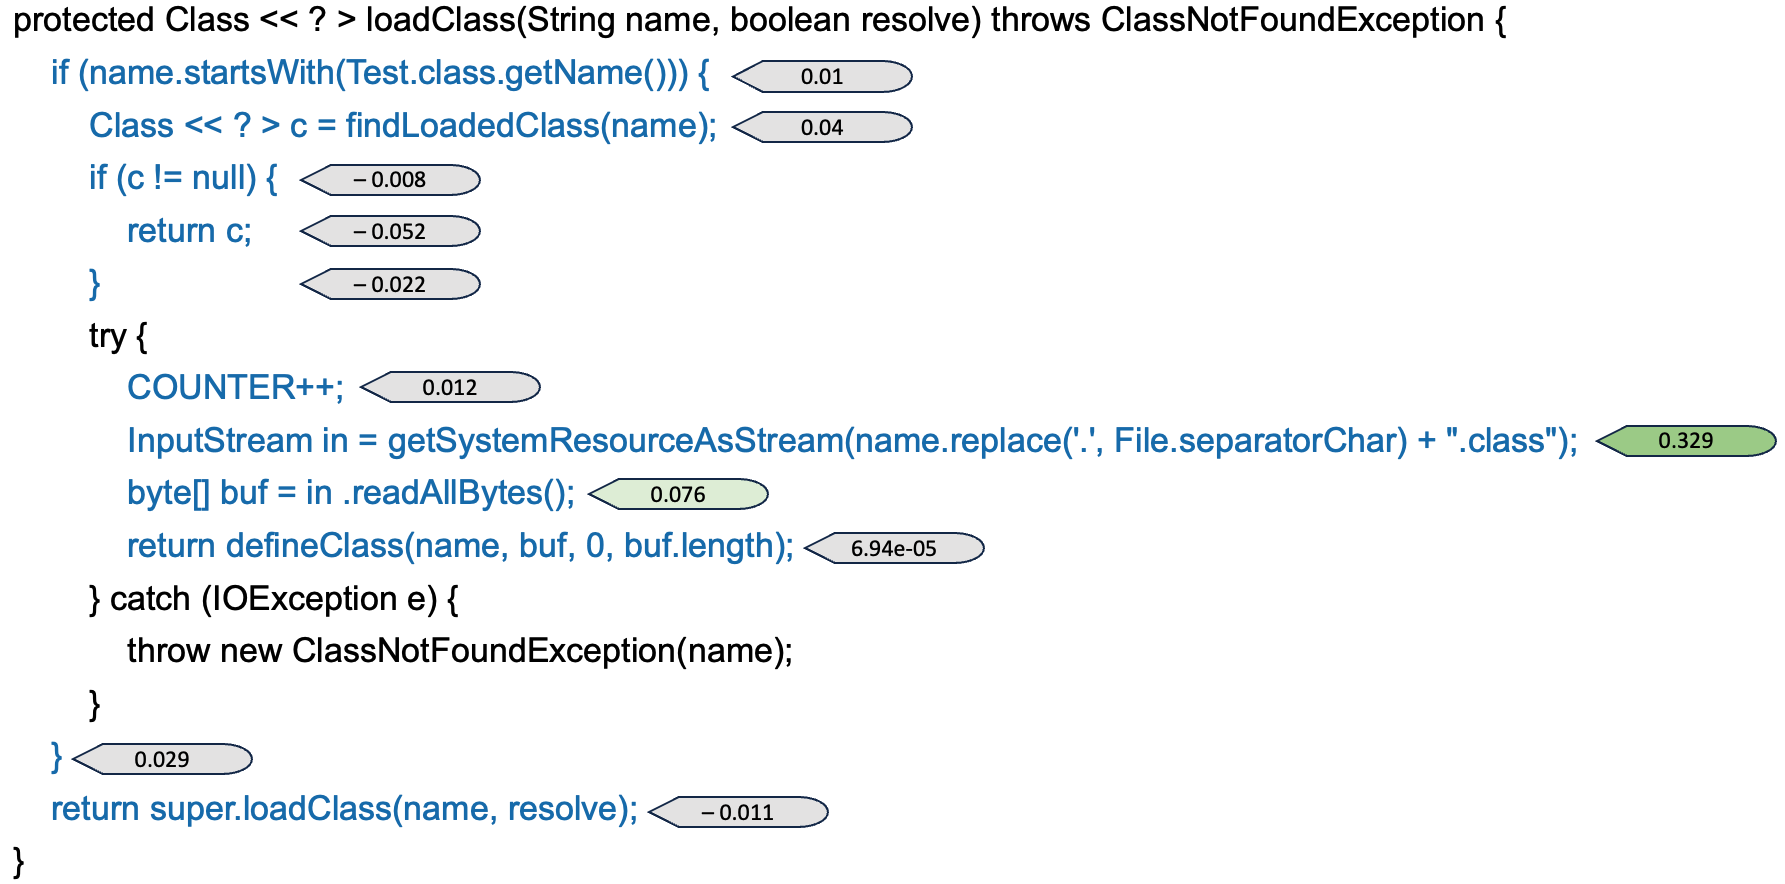
\includegraphics[width=3.4in]{rq1-case-study.png}
        \vspace{-20pt}
 	\caption{{\xblock} Case Study}
 	\label{fig:rq1-case}	
\end{figure}

\noindent {\bf Attribution Scores.} To illustrate how {\xblock} makes
the prediction, in Figure~\ref{fig:rq1-case}, we shows a code snippet
that catches an \code{IOException} thrown by the \code{readAllBytes}
API call on an \code{InputStream} object. CodeBERT produces as a
by-product an {\em attribution score} for each code sub-token in the
input. The higher the score of a token the higher attention that the
model pays to that token, contributing to the prediction result. In
Figure~\ref{fig:rq1-case}, for each statement, we show the statement
attribution score, which is calculated by averaging the attribution
scores of all the sub-tokens in the statement.
%The number after each statement is the statement attribution score,
%which is calculated by averaging the attribution scores of all the
%sub-tokens in the statement.
%
A positive attribution score means that the statement contributes
positively to the model's predicted class, while a negative score
means the statement contributes negatively to the predicted class.
As seen, the two statements that receive the highest scores are the
statement that defines the \code{InputStream} variable and the
statement that invokes the \code{readAllBytes} method call on the
\code{InputStream} object. This example illustrates that the model
is able to put the attention on the right (sub)token
of the input to decide the need of the \code{try-catch} block.


\begin{table}[t]%[htpb]
  \caption{Try-Catch Necessity Checking Evaluated On Test Partitions by The Number Of Try-Catch Blocks (RQ1) }
  \vspace{-12pt}
  \small
	\begin{center}
		\renewcommand{\arraystretch}{1}
		\begin{tabular}{| p{1.0cm}<{\centering} | p{0.7cm}<{\centering} | p{0.7cm}<{\centering}| p{0.7cm}<{\centering} | p{0.7cm}<{\centering} | p{0.7cm}<{\centering} | p{0.7cm}<{\centering} | }
		  \hline
			\multirow{2}{*}{} & \multicolumn{6}{c|}{Number of Try-Catch Blocks (Github Dataset)} \\
			\cline{2-7}
			  & Zero  & One & Two & Three & Four & Five\\
			\hline
			Precision & 0.0 &  1.0 & 1.0 & 1.0 & 1.0 & 1.0\\
			\hline
			Recall   & 0.0 &  0.9829 & 0.9988 & 1.0 & 0.9861 & 1.0\\
			\hline
			F1   & 0.0  &  0.9914 & 0.9994 & 1.0 & 0.9930 & 1.0\\
			\hline
		\end{tabular}
		\label{tab:rq1-detailed-result}
	\end{center}
\end{table}

In addition, we partitioned the test dataset according to the number
of \code{try-catch} blocks, and evaluated {\xblock} on each
partition. As seen in Table~\ref{tab:rq1-detailed-result}, {\xblock}
gives 100\% correct prediction on the partitions with zero, three and
five \code{try-catch} blocks. Moreover, it achieves 100\% precision
and above 0.99 F1-score across all the partitions, showing that
{\xblock}'s prediction ability remains strong regardless of the number
of \code{try-catch} blocks in a code snippet.

%With a Precision of 68\%, it can decide correctly
%2 out of 3 cases if a code snippet needs a \code{try-catch}
%block or not. With a Recall of 79\%, {\tool} covers 4 out of
%5 cases that needs to be placed in a \code{try-catch} block. Users
%just need to find 1 out of 5 cases. As a result, it achieves a high
%F-score of 0.73.
%In FuzzyCatch dataset, {\tool} also achieves a high level of
%performance with XX\% precision, YY\% recall, and ZZ\% F-score.

%the state-of-the-art approach, XRank, {\bf -7.1\%} in Recall, {\bf
%  28.3\%} in Precision, and {\bf 12.3\%} in F-score.

%In FuzzyCatch dataset, the relative improvements are XX\%, YY\%, and
%ZZ\% in precision, recall, and F-score, respectively.

%We examined closely the cases that {\tool} performed better than
%XRank.

%Examining the result, we reported the following. First, if the
%association score of {\em only one API method} in the snippet and {\em one
%exception} is higher than a threshold, XRank decides that a
%\code{try-catch} block is needed.  Thus, it often tends to output
%  ``Yes''. {\em Its recall is slightly
%  better, but precision is just marginally better than a coin toss
%  (0.53) in our balanced dataset. That leads to lower F-score than {\tool}}.
%%
%Second,
%%XRank relies on the association scores between the presence of
%%API method calls and the presence of a \code{try-catch} block.
%the decisions on the necessity of a \code{try-catch} block or the
%exception types depend on the pre-defined thresholds in XRank on those
%association scores. Thus, those pre-defined thresholds might not be
%suitable across the libraries. Third, for the incomplete code
%snippets in which the names of the API methods in different packages
%or libraries are the same (e.g., \code{toString} or \code{getText} in
%various JDK packages), XRank cannot distinguish them and use one entry
%in the dictionary for them due to its IR approach. In contrast, unlike
%XRank which considers only the API method calls in a \code{try-catch}
%block, {\tool} considers the code in the block as the context to learn
%the program dependencies/relations among the names of those API
%elements. That is, it leverages the relations among the names of API
%elements to learn their identities, thus, deciding better the need of
%\code{try-catch} blocks and the corresponding exception types.

%Tien:RQ2 Table
%\begin{table}[t]
%  \caption{Try-Catch Statement Detection Effectiveness (RQ2)}
%  \vspace{-12pt}
%	\begin{center}
%		\small
%		\renewcommand{\arraystretch}{1} 
%		\begin{tabular}{p{0.8cm}<{\centering}|p{0.4cm}<{\centering}|p{0.4cm}<{\centering}|p{0.4cm}<{\centering}|p{0.4cm}<{\centering}|p{0.4cm}<{\centering}|p{0.4cm}<{\centering}|p{0.4cm}<{\centering}|p{0.4cm}<{\centering}|p{0.4cm}<{\centering}|p{0.4cm}<{\centering}}
%			\hline
%			 	&  \multicolumn{10}{c}{Accuracy} \\
%			\cline{2-11}
%			     	&  N1  & N2   &  N3  & N4   &N5    & N6   &N7    & N8   &N9    & N10 \\
%			\hline
%			\tool     & 0.42 & 0.47 & 0.59 & 0.66 & 0.71 & 0.74 & 0.76 & 0.77 & 0.78  & 0.79  \\
%			\hline
%		\end{tabular}
%		Nx is number of nodes in the explanation
%                sub-graph (\code{try-catch} block)
%		\label{tab:rq2}
%	\end{center}
%\end{table}


%Take as an example a code snippet (not shown) in our dataset with the
%presence of \code{getText}. This name is popular with a very large number
%of API method candidates.
%%For example, in a code snippet, \code{getText} has a very large number
%%of API method candidates.
%However, considering the relation between \code{css} and
%\code{getText} in the code \code{`...css()\-.getText()'},~the number
%of candidates for \code{getText} is only 4. Finally, considering~the
%return value of \code{getText} as an argument of
%\code{setInnerText(...)} in the code
%\code{`setInnerText(...css()\-.getText())'}, only one candidate is
%remained:
%\code{com\-.google\-.gwt\-.resources\-.client\-.CssResource\-.getText()}.
%Thus, those relations actually help identify the API elements,
%leading to better decision in {\tool} on the \code{try-catch} block
%and exception types.
%%
%Because it has not seen any \code{try-catch} block involving
%\code{com\-.....getText()} and those related ones, {\tool} decides
%that the code snippet does not need a \code{try-catch} block. In
%contrast, XRank considers only the {\em pairwise} associate scores
%between an {\em individual API method call} and the exception types
%in a \code{catch} clause. It disregards those above
%relations/dependencies among the API names. Thus, it might
%misunderstand that \code{getText} needs a \code{try-catch} due to the
%co-occurrences of other API elements that need one. That is, without
%the dependencies, XRank might make incorrect identification of the API
%elements via their names, leading to incorrect exception
%recommendation.

%considering Groum but only to get better API ...


%\begin{table}[htpb]
%  \caption{Try-Catch Necessity Checking Comparison (RQ1)}
%  \vspace{-12pt}
%	\begin{center}
%		\renewcommand{\arraystretch}{1}
%		\begin{tabular}{p{1.5cm}<{\centering}|p{1.25cm}<{\centering}p{1.25cm}<{\centering}|p{1.25cm}<{\centering}p{1.25cm}<{\centering}}
%			\hline
%			\multirow{2}{*}{} & \multicolumn{2}{c|}{{\tool} Dataset} & \multicolumn{2}{c}{FuzzyCatch Dataset}\\
%			\cline{2-5}
%			  & \tool  & XRank & \tool  & XRank\\
%			\hline
%			Recall    & \textbf{0.81} & &&\\
%			Precision & \textbf{0.66} & &&\\
%			F-score   & \textbf{0.73} & &&\\
%			\hline
%		\end{tabular}
%		\label{tab:xblock}
%	\end{center}
%\end{table}

\subsection{RQ2. Try-Catch Block Detection Comparison Study}
\label{sec:rq2}

\begin{table}[t]
	\caption{RQ2. Try-Catch Block Detection Performance Comparison}
	\begin{center}
		\small
		\renewcommand{\arraystretch}{1} 
		\begin{tabular}{p{0.8cm}<{\centering}|p{0.4cm}<{\centering}|p{0.4cm}<{\centering}|p{0.4cm}<{\centering}|p{0.4cm}<{\centering}|p{0.4cm}<{\centering}|p{0.4cm}<{\centering}|p{0.4cm}<{\centering}|p{0.4cm}<{\centering}|p{0.4cm}<{\centering}|p{0.4cm}<{\centering}}
			\hline
			 	&  \multicolumn{10}{c}{Accuracy} \\
			\cline{2-11}
			     	&  N1  & N2   &  N3  & N4   &N5    & N6   &N7    & N8   &N9    & N10 \\
			\hline
			\tool       &  &  &  &  &  & 0.76 &  &  &  &   \\
			\hline
		\end{tabular}
		Nx: x is the number of nodes in the sub-graph (try-catch block)
		\label{RQ2_results}
	\end{center}
\end{table}

{\color{red}{N1-N10 are the number of nodes that the subgraph contains which means the size of the try-catch block. Because the average size of the try-catch is 5.7, I currently pick 6 as the size of the try-catch block. The accuracy here is defined as: if a statement is in the try-catch block and our model put it in the subgraph, I regard it is correct $S_c$. All other conditions, I think they are incorrect. If there are $S$ statements in the try-catch block, the total accuracy is calculated as $S_c/S$}}
\subsection{RQ3. Effectiveness on Exception Type Recommendation}
\label{sec:rq3}


\begin{table}[t]
	\caption{RQ3. Detailed Performance Comparison on Different \# of Statements in an Oracle Try-Catch Block (Recall)}
	\tabcolsep 2pt
	{\small
		\begin{center}
			\renewcommand{\arraystretch}{1}
			\begin{tabular}{p{3cm}<{\centering}|p{2cm}<{\centering}|p{2cm}<{\centering}}
				\hline
				\# ET in Oracle Block& Metrics& {\textsc{\tool}\xspace} \\
				\hline
				\multirow{1}{*}{1 (40376)}   & Hit-1  & 25841 (64\%) \\
				\hline
				\multirow{2}{*}{2 (2634)}  & Hit-1   & 2028 (77\%) \\
				& Hit-2         &  1081 (41\%) \\
				\hline
				\multirow{3}{*}{3 (547)}  & Hit-1    & 334 (61\%) \\
				& Hit-2     & 181 (33\%)\\
				& Hit-3     & 115 (21\%) \\
				\hline
				\multirow{4}{*}{3+ (391)}  & Hit-1   & 233 (59\%) \\
				& Hit-2     & 134 (35\%) \\
				& Hit-3     & 65 (17\%))\\
				\hline
			\end{tabular}		
		ET: Exception types
			\label{RQ3_results_1}
		\end{center}
	}
\end{table}

{\color{red}{1. Our model do well on hit-1 condition which means in most cases, our model can at least predict one exception type correctly for a try-catch block. 2. Results show that the more exception types one try-catch block has, our model is harder to predict all of them correctly. }}


\begin{table}[t]
	\caption{RQ3. Detailed Performance Comparison on Different \# of Statements in a Predicted Try-Catch Block (Precision)}
	\vspace{-10pt}
	\tabcolsep 2pt
	{\small
		\begin{center}
			\renewcommand{\arraystretch}{1}
			\begin{tabular}{p{3cm}<{\centering}|p{2cm}<{\centering}|p{2cm}<{\centering}}
				\hline
				\# ET in Predicted Block & Metrics & {\textsc{\tool}\xspace} \\
				\hline
				\multirow{1}{*}{1 (36995)}   & Hit-1  & 13589 (37\%) \\
				\hline
				\multirow{2}{*}{2 (4981)}  & Hit-1   & 1594 (32\%) \\
				& Hit-2       						& 947 (19\%) \\
				\hline
				\multirow{3}{*}{3 (1972)}  & Hit-1    & 611 (31\%) \\
				& Hit-2         					& 458 (23\%)\\
				& Hit-3         				  	& 185 (9\%) \\
				\hline
			\end{tabular}
		ET: Exception types
			\label{RQ3_results_2}
		\end{center}
	}
\end{table}
\subsection{Ablation Study (RQ4)}
\label{sec:rq4}



\begin{table}[t]
  \caption{RQ4. Impact of Different Features on {\xblock}}
    %Try-Catch Block Necessity Checking}
  \vspace{-12pt}
  \begin{center}
    \small
		\renewcommand{\arraystretch}{1}
		\begin{tabular}{p{1.75cm}<{\centering}|p{1.75cm}<{\centering}|p{1.75cm}<{\centering}|p{1.75cm}<{\centering}}
			\hline
			  & \tool w/o SOT & \tool w/o AST & \tool \\
			\hline
			Recall    & & & \textbf{0.81} \\
			Precision & & &\textbf{0.66} \\
			F-score   & & &\textbf{0.73} \\
			\hline
		\end{tabular}
		SOT: Sequence of tokens; AST: Abstract Syntax Tree
		\label{tab:sensi-xblock}
	\end{center}
\end{table}

\subsubsection{Impact of Different Features on Try-Catch Block Necessity Checking ({\xblock})}

Table~\ref{tab:sensi-xblock} displays the results when we removed the
two key features in {\tool} and measured {\xblock}'s performance. As
seen, without the sequences of code (lexical tokens) for each
statement, Recall, Precision, and F-score decrease XX\%, YY\%, and
ZZ\%, respectively. Without considering the AST structure, Recall,
Precision, and F-score also decrease even further with XX\%, YY\%, and
ZZ\%, respectively. In other words, the code structure has a higher
contribution than the lexical values of code tokens.


%{\color{red}{Without sequence of tokens or AST in try-catch block necessity checking will lead to the reduce of results. Once I finish this sensitivity experiments, I will update this table. }}

\begin{table}[t]
  \caption{RQ4. Impact of Different Features on {\xstate}}
  \vspace{-12pt}
    %\code{Try-catch} Statement Prediction}
  \small
	\begin{center}
		\renewcommand{\arraystretch}{1}
		\begin{tabular}{p{1.75cm}<{\centering}|p{1.75cm}<{\centering}|p{1.75cm}<{\centering}|p{1.75cm}<{\centering}}
			\hline
			  & \tool w/o SOT & \tool w/o AST & \tool \\
			\hline
			Accuracy    & & & \textbf{0.76} \\
			\hline
		\end{tabular}
		SOT: Sequence of tokens; AST: Abstract syntax tree
		\label{tab:sensi-xstate}
	\end{center}
\end{table}

\subsubsection{Impact of Different Features on Try-Catch Statement Detection ({\xstate})}

%Table~\ref{tab:sensi-xstate} displays the results when we removed the
%two key features in {\tool} and measured the performance of {\xstate}.
We used six as the limit on the number of nodes in the explanation
sub-graph in which {\tool} achieves 0.76 of Accuracy. Note: the
average number of the statements in a \code{try-catch} block in our
dataset is 5.7. As seen, the result in Table~\ref{tab:sensi-xstate} is
consistent with Table~\ref{tab:sensi-xblock}, as AST contributes
slightly more than code sequences.

%without the sequences of code (lexical tokens) for each statement,
%Accuracy decreases XX\%. Without considering the AST structure,
%Accuracy also decreases even further with XX\%. In other words, the
%code structure has a higher contribution than the lexical values of
%code tokens.

\subsubsection{Impact of Different Features on Exception Type Recommendation ({\xtype})}

Tables~\ref{tab:sensi-xtype-recall}
and~\ref{tab:sensi-xtype-precision} display the results. As seen, the
impact result is consistent with those in
Tables~\ref{tab:sensi-xblock} and~\ref{tab:sensi-xstate}.
Thus, code structure has slightly higher impact than code sequence.

%when we removed the two key features in {\tool} and measured the
%performance of {\xtype}. As seen, without the sequences of code
%(lexical tokens) for each statement, all the evaluation metrics
%\code{Hit}-$n$ decrease across the board in both recall and
%precision. Without considering the AST structure, all the evaluation
%metrics decrease slightly further.  Thus, this result is consistent
%with the above results as the code structure has a higher contribution
%than the lexical values of code tokens.

\begin{table}[t]
  \caption{Impact of Different Features on {\xtype} (Recall)}
  \vspace{-12pt}
	\tabcolsep 2pt
	{\small
		\begin{center}
			\renewcommand{\arraystretch}{1}
			\begin{tabular}{p{2cm}<{\centering}|p{1cm}<{\centering}|p{1.5cm}<{\centering}|p{1.5cm}<{\centering}|p{1.5cm}<{\centering}}
				\hline
				\# ET in \code{Try-Catch} Block in Oracle & Metrics &{\textsc{\tool w/o SOT}\xspace}&{\textsc{\tool w/o AST}\xspace}& {\textsc{\tool}\xspace} \\
				\hline
				\multirow{1}{*}{1 (40376)}   & Hit-1  &&& 25,841 (64\%) \\
				\hline
				\multirow{2}{*}{2 (2634)}  & Hit-1   &&& 2,028 (77\%) \\
				& Hit-2         &&&  1081 (41\%) \\
				\hline
				\multirow{3}{*}{3 (547)}  & Hit-1    &&& 334 (61\%) \\
				& Hit-2     &&& 181 (33\%)\\
				& Hit-3     &&& 115 (21\%) \\
				\hline
				\multirow{4}{*}{3+ (391)}  & Hit-1   &&& 233 (59\%) \\
				& Hit-2     &&& 134 (35\%) \\
				& Hit-3     &&& 65 (17\%)\\
				\hline
			\end{tabular}
		ET:Exception types; SOT: Sequence of tokens; AST: Abstract syntax tree		
			\label{tab:sensi-xtype-recall}
		\end{center}
	}
\end{table}

\begin{table}[t]
	\caption{Impact of Different Features on {\xtype} (Precision)}
	\vspace{-10pt}
	\tabcolsep 2pt
	{\small
		\begin{center}
			\renewcommand{\arraystretch}{1}
			\begin{tabular}{p{2cm}<{\centering}|p{1cm}<{\centering}|p{1.5cm}<{\centering}|p{1.5cm}<{\centering}|p{1.5cm}<{\centering}}
				\hline
				\# ET in Predicted \code{Try-Catch} Block & Metrics &{\textsc{\tool w/o SOT}\xspace}&{\textsc{\tool w/o AST}\xspace}& {\textsc{\tool}\xspace} \\
				\hline
				\multirow{1}{*}{1 (36995)}   & Hit-1  &&& 13,589 (37\%) \\
				\hline
				\multirow{2}{*}{2 (4981)}  & Hit-1   &&& 1,594 (32\%) \\
				& Hit-2       						&&& 947 (19\%) \\
				\hline
				\multirow{3}{*}{3 (1972)}  & Hit-1   && & 611 (31\%) \\
				& Hit-2         					&&& 458 (23\%)\\
				& Hit-3         				  	&&& 185 (9\%) \\
				\hline
			\end{tabular}
		ET: Exception types; SOT: Sequence of tokens; AST: Abstract syntax tree
			\label{tab:sensi-xtype-precision}
		\end{center}
	}
\end{table}

%{\color{red}{Without sequence of tokens or AST in exception type prediction will lead to the reduce of results of all hit-1, hit-2, and hit-3. Once I finish this sensitivity experiments, I will update these two table. }}


%%%\begin{table}[t]
%%%	\caption{RQ4. Impact of the \# Limit of Exception Type on Exception Type Prediction (Recall)}
%%%	\tabcolsep 2pt
%%%	{\small
%%%		\begin{center}
%%%			\renewcommand{\arraystretch}{1}
%%%			\begin{tabular}{p{3.5cm}<{\centering}|p{2cm}<{\centering}|p{2.5cm}<{\centering}}
%%%				\hline
%%%				\# ET in Oracle Block& Metrics& {\textsc{\tool}\xspace} \\
%%%				\hline
%%%				\multirow{1}{*}{1 (40376)}   & Hit-1  & 27867 (69\%) \\
%%%				\hline
%%%				\multirow{2}{*}{2 (2634)}  & Hit-1   & 2131 (81\%) \\
%%%				& Hit-2         &  1162 (44\%) \\
%%%				\hline
%%%				\multirow{3}{*}{3 (547)}  & Hit-1    & 353 (64\%) \\
%%%				& Hit-2     & 189 (35\%)\\
%%%				& Hit-3     & 142 (26\%) \\
%%%				\hline
%%%				\multirow{4}{*}{4 (267)}  & Hit-1   & 175 (65\%) \\
%%%				& Hit-2     & 107 (40\%) \\
%%%				& Hit-3     & 55 (21\%))\\
%%%				& Hit-4     & 21 (8\%))\\
%%%				\hline
%%%				\multirow{4}{*}{4+ (124)}  & Hit-1   & 77 (62\%) \\
%%%				& Hit-2     & 46 (38\%) \\
%%%				& Hit-3     & 21 (17\%))\\
%%%				& Hit-4     & 5 (4\%))\\
%%%				\hline
%%%			\end{tabular}		
%%%			ET: Exception types
%%%			\label{RQ4_results_4}
%%%		\end{center}
%%%	}
%%%\end{table}

%%%\begin{table}[t]
%%%	\caption{RQ4. Impact of the \# Limit of Exception Type on Exception Type Prediction (Precision)}
%%%	\vspace{-10pt}
%%%	\tabcolsep 2pt
%%%	{\small
%%%		\begin{center}
%%%			\renewcommand{\arraystretch}{1}
%%%			\begin{tabular}{p{3.5cm}<{\centering}|p{2cm}<{\centering}|p{2.5cm}<{\centering}}
%%%				\hline
%%%				\# ET in Predicted Block & Metrics & {\textsc{\tool}\xspace} \\
%%%				\hline
%%%				\multirow{1}{*}{1 (34707)}   & Hit-1  & 11113 (32\%) \\
%%%				\hline
%%%				\multirow{2}{*}{2 (5892)}  & Hit-1   & 1829 (31\%) \\
%%%				& Hit-2       						& 764 (13\%) \\
%%%				\hline
%%%				\multirow{3}{*}{3 (2321)}  & Hit-1    & 654 (28\%) \\
%%%				& Hit-2         					& 437 (19\%)\\
%%%				& Hit-3         				  	& 159 (7\%) \\
%%%				\hline
%%%				\multirow{4}{*}{4 (1028)}  & Hit-1    & 268 (26\%) \\
%%%				& Hit-2         					& 211 (21\%)\\
%%%				& Hit-3         				  	& 94 (9\%) \\
%%%				& Hit-4         				  	& 33 (3\%) \\
%%%				\hline
%%%			\end{tabular}
%%%			ET: Exception types
%%%			\label{RQ4_results_5}
%%%		\end{center}
%%%	}
%%%\end{table}



\section{Related Work}
\label{sec:related}

The automated approaches to recommend exception handling can be
classified into four categories as presented in Section~\ref{sec:intro}.
%The first category of approaches defines the {\em heuristics} on
%exception types, API calls, and variable types to recommend proper
%exception handling~\cite{barbosa-bsse12}.
%%These heuristic-based approaches do not always work in all the cases
%%and need to be updated for the new/updated API elements or a new
%%library. To address the heuristics,
%The second category of approaches relied on the enforced {\em
%  exception handling policies}~\cite{barbosa-tse16,barbosa-saner18}.
%%Exception policies are defined via domain-specific
%%language~\cite{barbosa-tse16}.
%%Exception Policy Expert (EPE)~\cite{barbosa-saner18} is a tool
%%embedded in Eclipse IDE that warns developers about exception policy
%%violations. The drawback of this category is the hard-code of the
%%policies in the EPE tool.
%%To overcome the pre-defined exception handling policies,
%The third category of approaches aim to {\em mine the frequent
%  exception handling} code from a large corpus. These mining
%approaches~\cite{chanchal-scam14} provide more flexibility than policy
%enforcement.
%%They rely on the idea that similar code has similar exception
%%handling. As with mining, these approaches face the challenge of
%%deterministically setting the threshold for similar code and similar
%%exception handling. In many cases, the two pieces of code are quite
%%different, yet have the same set of exceptions to be handled.
The closest work to {\tool} is the state-of-the-art {\em information
  retrieval} (IR) approaches~\cite{xrank-fse20}, which provides more
flexibility than the others. XRank~\cite{xrank-fse20} recommends a
ranked list of API calls that might need exception handling and
XHand~\cite{xrank-fse20} recommends exception handling code. Both
leverages fuzzy set theory to compute the associations between API
method calls and the exception types. This direction has three key
limitations. First, one needs to pre-define a threshold for feature
matching for the retrieval of API elements or exception types. Second,
the IR techniques are not flexible as the ML approaches because they
use the lexical values of API simple names. Thus, they suffer the
ambiguity in the names of API elements in incomplete code
snippets. Lastly, XRank/XHand considers only pairwise associations
between the API method calls and exceptions. It disregards the
surrounding code context and the dependencies/relations. XRank/XHand
simply uses Groum~\cite{fse09}, a dependency graph among API elements,
to collect the API calls, but did not use dependencies in
computing the association scores.
%among the API elements to disambiguate the simple names of the API
%elements.

In addition to exception handling recommendation research,
ThEx~\cite{throw-ase22} predict which exception(s) shall be thrown
under a given programming context. ThEx learns a classification model
from existing thrown exceptions in different contexts.

%The features include code information surrounding the thrown
%exceptions, such as the thrown locations and related variable names.



%\section{Conclusion}

{\tool} is the first neural-network model to automated exception
handling recommendation in three tasks for (in)complete code. It is
designed to capture the basic insights to overcome key limitations of
the state-of-the-art IR approaches. With the learning-based approach,
it does not rely on a pre-defined threshold for explicit feature
matching. Our empirical evaluation shows that the dependencies and
context help {\tool} learn the identities of API elements to avoid
name ambiguity and to learn their relations with the exception
types. Our results also demonstrate that {\tool} improves over the
state-of-the-art approaches in both intrinsic and extrinsic tasks
including exception-related bug detection.



%\section*{Acknowledgments}
%This work was supported in part by the US National Science Foundation
%(NSF) grants CNS-2120386, CCF-1723215, CCF-1723432, TWC-1723198, and
%the US National Security Agency (NSA) grant NCAE-C-002-2021 on
%Cybersecurity Research Innovation.

\newpage

\balance

%\bibliographystyle{plain}
%\bibliographystyle{ACM-Reference-Format}
\bibliographystyle{ACM-Reference-Format}

\bibliography{references, Reference, icse21IntVD, FL}

\end{document}

%\endinput
%%
%% End of file `sample-sigconf.tex'.
